%%%%%%%% ICML 2023 EXAMPLE LATEX SUBMISSION FILE %%%%%%%%%%%%%%%%%

\documentclass[table]{article}

% Recommended, but optional, packages for figures and better typesetting:
\usepackage{microtype}
\usepackage{graphicx}
\usepackage{subfigure}
\usepackage{booktabs} % for professional tables

% hyperref makes hyperlinks in the resulting PDF.
% If your build breaks (sometimes temporarily if a hyperlink spans a page)
% please comment out the following usepackage line and replace
% \usepackage{icml2023} with \usepackage[nohyperref]{icml2023} above.
\usepackage{hyperref}


% Attempt to make hyperref and algorithmic work together better:
\newcommand{\theHalgorithm}{\arabic{algorithm}}

% Use the following line for the initial blind version submitted for review:
% \usepackage{icml2023}

% If accepted, instead use the following line for the camera-ready submission:
\usepackage[preprint]{icml2025}

% For theorems and such
\usepackage{amsmath}
\usepackage{amssymb}
\usepackage{mathtools}
\usepackage{amsthm}
\usepackage{tikz}
\usepackage{algorithm}
\usepackage{algorithmic}
% if you use cleverer.
\usepackage[capitalize,noabbrev]{cleveref}

%%%%%%%%%%%%%%%%%%%%%%%%%%%%%%%%
% THEOREMS
%%%%%%%%%%%%%%%%%%%%%%%%%%%%%%%%
\theoremstyle{plain}
\newtheorem{theorem}{Theorem}[section]
\newtheorem{proposition}[theorem]{Proposition}
\newtheorem{lemma}[theorem]{Lemma}
\newtheorem{corollary}[theorem]{Corollary}
\newtheorem{fact}[theorem]{Fact}
\theoremstyle{definition}
\newtheorem{definition}[theorem]{Definition}
\newtheorem{assumption}[theorem]{Assumption}
\newtheorem{example}[theorem]{Example}
\newtheorem{remark}[theorem]{Remark}
\newtheorem{note}[theorem]{Note}
\newtheorem{claim}[theorem]{Claim}
\theoremstyle{remark}



% Todonotes is useful during development; simply uncomment the next line
%    and comment out the line below the next line to turn off comments
%\usepackage[disable,textsize=tiny]{todonotes}
\usepackage[textsize=tiny]{todonotes}

%%%%% NEW MATH DEFINITIONS %%%%%

% \usepackage{amsmath,amsfonts,bm}
\usepackage{amsmath,amsfonts}

\usepackage{pifont}


\newcommand{\R}{\mathbb{R}}


\def\va{{\mathbf{a}}}
\def\vg{{\mathbf{g}}}

% Sets
\def\sR{\mathbb{R}}
\def\sC{\mathbb{C}}
\def\sZ{\mathbb{Z}}
\def\sN{\mathbb{N}}
\def\sQ{\mathbb{Q}}

\def\sS{\mathcal{S}}



% Vectors
\def\vzero{{\mathbf{0}}}
\def\vone{{\mathbf{1}}}
\def\vmu{{\mathbf{\mu}}}
\def\vtheta{{\mathbf{\theta}}}
\def\va{{\mathbf{a}}}
\def\vb{{\mathbf{b}}}
\def\vc{{\mathbf{c}}}
\def\vd{{\mathbf{d}}}
\def\ve{{\mathbf{e}}}
\def\vf{{\mathbf{f}}}
\def\vg{{\mathbf{g}}}
\def\vh{{\mathbf{h}}}
\def\vi{{\mathbf{i}}}
\def\vj{{\mathbf{j}}}
\def\vk{{\mathbf{k}}}
\def\vl{{\mathbf{l}}}
\def\vm{{\mathbf{m}}}
\def\vn{{\mathbf{n}}}
\def\vo{{\mathbf{o}}}
\def\vp{{\mathbf{p}}}
\def\vq{{\mathbf{q}}}
\def\vr{{\mathbf{r}}}
\def\vs{{\mathbf{s}}}
\def\vt{{\mathbf{t}}}
\def\vu{{\mathbf{u}}}
\def\vv{{\mathbf{v}}}
\def\vw{{\mathbf{w}}}
\def\vx{{\mathbf{x}}}
\def\vy{{\mathbf{y}}}
\def\vz{{\mathbf{z}}}
\def\vzeta{{\mathbf{\zeta}}}

% Matrix
\def\mA{{\mathbf{A}}}
\def\mB{{\mathbf{B}}}
\def\mC{{\mathbf{C}}}
\def\mD{{\mathbf{D}}}
\def\mE{{\mathbf{E}}}
\def\mF{{\mathbf{F}}}
\def\mG{{\mathbf{G}}}
\def\mH{{\mathbf{H}}}
\def\mI{{\mathbf{I}}}
\def\mJ{{\mathbf{J}}}
\def\mK{{\mathbf{K}}}
\def\mL{{\mathbf{L}}}
\def\mM{{\mathbf{M}}}
\def\mN{{\mathbf{N}}}
\def\mO{{\mathbf{O}}}
\def\mP{{\mathbf{P}}}
\def\mQ{{\mathbf{Q}}}
\def\mR{{\mathbf{R}}}
\def\mS{{\mathbf{S}}}
\def\mT{{\mathbf{T}}}
\def\mU{{\mathbf{U}}}
\def\mV{{\mathbf{V}}}
\def\mW{{\mathbf{W}}}
\def\mX{{\mathbf{X}}}
\def\mY{{\mathbf{Y}}}
\def\mZ{{\mathbf{Z}}}
\def\mBeta{{\mathbf{\beta}}}
\def\mPhi{{\mathbf{\Phi}}}
\def\mLambda{{\mathbf{\Lambda}}}
\def\mSigma{{\mathbf{\Sigma}}}


% Expectation
% \def\eE{\mathop{\mathbb{E}}\limits}
\def\eE{\mathbb{E}}

% Probability
\def\pP{\mathbb{P}}

% Tilde
\def\tf{\tilde{f}}
\def\tS{\tilde{S}}
\def\wtF{\widetilde{\mathcal{F}}}
\def\whR{\widehat{R}}
\def\tvx{\tilde{\mathbf{x}}}
\def\ty{\tilde{y}}


\def\defeq{\overset{\textup{def}}{=}}
% \def\defeq{\overset{.}{=}}
\def\defone{\overset{\text{\ding{172}}}{=}}
\def\deftwo{\overset{\text{\ding{173}}}{=}}
\def\leqone{\overset{\text{\ding{172}}}{\leq}}
\def\leqtwo{\overset{\text{\ding{173}}}{\leq}}
\def\leqthree{\overset{\text{\ding{174}}}{\leq}}
\def\leqfour{\overset{\text{\ding{175}}}{\leq}}
\def\eqone{\overset{\text{\ding{172}}}{=}}
\def\eqtwo{\overset{\text{\ding{173}}}{=}}
\def\eqthree{\overset{\text{\ding{174}}}{=}}
\def\eqfour{\overset{\text{\ding{175}}}{=}}
\def\geqfive{\overset{\text{\ding{176}}}{\geq}}
\newcommand*{\ldblbrace}{\{\mskip-5mu\{}
\newcommand*{\rdblbrace}{\}\mskip-5mu\}}
\newcommand*{\Ldblbrace}{\left\{\mskip-7mu\left\{}
\newcommand*{\Rdblbrace}{\right\}\mskip-7mu\right\}}
\newcommand*{\dis}{{\operatorname{dis}}}
\newcommand*{\disR}{\operatorname{dis}^\mathsf{R}}
\newcommand*{\disH}{\operatorname{dis}^\mathsf{H}}
\newcommand*{\hash}{\mathsf{hash}}
\newcommand*{\op}{\mathsf{op}}
\newcommand*{\agg}{\mathsf{agg}}
\newcommand*{\walk}{\mathsf{walk}}
\newcommand*{\pool}{\mathsf{Pool}}
\newcommand*{\twist}{\mathsf{twist}}
\newcommand*{\meta}{\mathsf{Meta}}
\newcommand*{\DKL}[2]{\KL(#1\|#2)}
\newcommand*{\DEP}{\operatorname{DEP}}
\newcommand*{\SEP}{\operatorname{SEP}}
\newcommand*{\NEW}{\operatorname{NEW}}
\newcommand*{\PPL}{\operatorname{TER}}
\newcommand*{\SER}{\operatorname{SER}}
\newcommand*{\PROC}{\operatorname{REVR}}
\newcommand*{\mask}{\texttt{[m]}}
\newcommand*{\MK}[1]{\textcolor{red}{[Mark: #1]}}
\newcommand*{\guhao}[1]{\textcolor{blue}{[guhao: #1]}}
\newcommand*{\yihan}[1]{\textcolor{purple}{[yihan: #1]}}
\newcommand{\TO}{\textbf{ to }}
\newcommand{\RETURN}{\STATE \textbf{return} }
\usepackage{enumitem}
\usepackage{makecell}
\usepackage{multirow}
\usepackage{mathrsfs}
% \usepackage[table]{xcolor}

% The \icmltitle you define below is probably too long as a header.
% Therefore, a short form for the running title is supplied here:
\icmltitlerunning{Theoretical Benefit and Limitation of Diffusion Language Model}

\begin{document}

\twocolumn[
\icmltitle{Theoretical Benefit and Limitation of Diffusion Language Model}

% It is OKAY to include author information, even for blind
% submissions: the style file will automatically remove it for you
% unless you've provided the [accepted] option to the icml2023
% package.

% List of affiliations: The first argument should be a (short)
% identifier you will use later to specify author affiliations
% Academic affiliations should list Department, University, City, Region, Country
% Industry affiliations should list Company, City, Region, Country

% You can specify symbols, otherwise they are numbered in order.
% Ideally, you should not use this facility. Affiliations will be numbered
% in order of appearance and this is the preferred way.
\icmlsetsymbol{equal}{*}

\vspace{-3pt}
\begin{icmlauthorlist}
\icmlauthor{Guhao Feng}{equal,pku}
\icmlauthor{Yihan Geng}{equal,pku}
\icmlauthor{Jian Guan}{ant}
\icmlauthor{Wei Wu}{ant}
\icmlauthor{Liwei Wang}{pku}
\icmlauthor{Di He}{pku}
\end{icmlauthorlist}
\icmlaffiliation{pku}{Peking University}
\icmlaffiliation{ant}{Ant Group}
% \icmlaffiliation{pku1}{National Key Laboratory of General Artificial Intelligence, School of Intelligence Science and Technology, Peking University}
% \icmlaffiliation{pku2}{Center for Data Science, Peking University}
% \icmlaffiliation{pku3}{School of Mathematical Sciences, Peking University}

% \icmlcorrespondingauthor{Guhao Feng}{fenguhao@stu.pku.edu.cn}
% \icmlcorrespondingauthor{Liwei Wang}{wanglw@cis.pku.edu.cn}
% \icmlcorrespondingauthor{Di He}{dihe@pku.edu.cn}


% You may provide any keywords that you
% find helpful for describing your paper; these are used to populate
% the "keywords" metadata in the PDF but will not be shown in the document
\icmlkeywords{Machine Learning, ICML}

\vskip 0.24in
]

% this must go after the closing bracket ] following \twocolumn[ ...

% This command actually creates the footnote in the first column
% listing the affiliations and the copyright notice.
% The command takes one argument, which is text to display at the start of the footnote.
% The \icmlEqualContribution command is standard text for equal contribution.
% Remove it (just {}) if you do not need this facility.

%\printAffiliationsAndNotice{}  % leave blank if no need to mention equal contribution
\printAffiliationsAndNotice{\icmlEqualContribution} % otherwise use the standard text.

\begin{abstract}
Diffusion language models have emerged as a promising approach for text generation. One would naturally expect this method to be an efficient replacement for autoregressive models since multiple tokens can be sampled in parallel during each diffusion step. However, its efficiency-accuracy trade-off is not yet well understood. In this paper, we present a rigorous theoretical analysis of a widely used type of diffusion language model, the Masked Diffusion Model (MDM), and find that its effectiveness heavily depends on the target evaluation metric. Under mild conditions, we prove that when using perplexity as the metric, MDMs can achieve near-optimal perplexity in sampling steps regardless of sequence length, demonstrating that efficiency can be achieved without sacrificing performance. However, when using the sequence error rate--which is important for understanding the ``correctness" of a sequence, such as a reasoning chain--we show that the required sampling steps must scale linearly with sequence length to obtain ``correct" sequences, thereby eliminating MDM's efficiency advantage over autoregressive models. Our analysis establishes the first theoretical foundation for understanding the benefits and limitations of MDMs. All theoretical findings are supported by empirical studies.
\end{abstract}

% 
% 
The widespread integration of communication networks and smart devices in modern control systems has increased the vulnerability of industrial systems to online cyber-attacks, e.g., Industroyer, Blackenergy, etc \citep{osti_1505628}.
% Modern control systems have seen a large push to include communication networks and smart devices to increase performance, made possible by improvements in communication device cost and energy consumption. This trend has been coupled with the usage of open-standard communication protocols among industrial control systems, making them vulnerable to online cyber-attacks such as Industroyer, Blackenergy, etc \citep{osti_1505628}. 
To counter this, methods have been developed to improve security by achieving attack detection, mitigation, and monitoring, among others \citep{sandberg2022secure}. This paper focuses on active attack diagnosis to mitigate stealthy attacks. 
%
%\subsection{Literature review}

Active diagnosis techniques rely on the inclusion of additional moduli to control systems
% inclusion within the control system of additional moduli 
to alter the behavior of the system compared to information known by the attacker. 
For instance, the concept of additive watermarking was introduced in \cite{mo2015physical}, where noise signals of known mean and variance are added at the plant and compensated for it at the controller. 
This compensation, however, is not exact, causing some performance degradation. Thus, trade-offs between performance and detectability  are necessary \citep{zhu2023detection}.
% A later work \citep{zhu2023detection} designs the watermark signal by trading performance for detection. Thus, although additive watermarking serves as a good detection scheme, they endure performance losses even in the nominal case. 

In encrypted control \citep{darup2021encrypted}, the sensor data is encrypted, sent to the controller, and then operated on directly. Encrypted input signals are sent back to the plant for decryption. Although encryption is widespread in IT security, in control systems it presents some concerns, such as the introduction of time delays \citep{stabile2024verifiable}, while it may present inherent weaknesses \citep{alisic2023model}.
% they are not preferred as they introduce time delays \citep{stabile2024verifiable} which can cause instability, and some encryption schemes can be very weak  \citep{alisic2023model}. 

In moving target defense \citep{griffioen2020moving}, the plant is augmented with fictitious dynamics, known to the controller. The plant output is transmitted to the controller along with the fictitious states over a network under attack. 
The additional measurements then aide in the detection of attacks. 
This comes at the cost of higher communication bandwidth needs, which increases rapidly with the dimension of the augmented systems.
% Since the dynamics of the fictitious dynamics are exactly known to the controller, the attack is detected easily. However, when the scale of the system increases, the communication bandwidth used by moving the target defense approach increases rapidly. 

Other recently proposed works include two-way coding \citep{fang2019two}, a weak encryuption technique, and dynamic masking \citep{abdalmoaty2023privacy}, which enhances privacy as well as security, have been shown to be effective against zero-dynamics attacks.
% Two-way coding \citep{fang2019two} and dynamic masking \citep{abdalmoaty2023privacy} are other recently proposed approaches. Two-way coding is another form of weak encryption technique whilst dynamic masking proposes an architecture that enhances both privacy and security. These schemes are shown to be effective against zero dynamics attacks but remain to be studied for other classes of attacks. 
% Recent extensions include \citep{mukherjee2021secure,ramos2024privacy}.
% Some other works which are related are \citep{mukherjee2021secure}, an extension of \cite{fang2019two}. The work \citep{ramos2024privacy} is an extension of moving target defense for multi-agent systems. 
Furthermore, filtering techniques for attack detection are proposed by \cite{murguia2020security,hashemi2022codesign,escudero2023safety}, while not focusing on stealthy attacks.
% The works \citep{murguia2020security,hashemi2022codesign,escudero2023safety} develop filtering techniques to guarantee safety, without being focused on stealthy covert attacks.

Multiplicative watermarking (mWM) has been proposed by the authors as a diagnosis technique \citep{ferrari2020switching}. mWM consists of a pair of filters on each communication channel between the plant and its controller; the scheme is affine to weak encryption, whereby ``encoding'' and ``decoding'' are done by changing signals' dynamic characteristics through inverse pairs of filters. This enables original signals to be recovered exactly, and thus does not lead to performance degradation.
% A multiplicative watermark is an affine to a weak encryption technique, through which the signal is ``encoded'' by a filter, changing its dynamic behavior. The use of inverse pairs means that the original signal can be recovered, through ``decoding'' via an inverse filter. As such, differently to techniques based on additive watermarking, no performance is lost due to the injection of noise, and there are no bandwidth limitations.

%\subsection{Contributions}
One of the critical features of multiplicative watermarking is that to detect stealthy attacks, the mWM filter parameters must be switched over time. In this paper, an algorithm to optimally design the mWM parameters after a switching event is presented, enhancing detection performance, without changing the switching time.
% This is done without changing the switching time, which is taken as given.

\textcolor{black}{
To formalize the filter design problem, we suppose the defender is interested in optimal performance against adversaries injecting covert attacks with matched system parameters \citep{smith2015covert}, including the mWM parameters prior to the switch. This scenario represents a worst case where malicious agents can take full control of the system while remaining undetected.
Thus, the attack strategy is explicitly included within the formulation of the closed-loop system, and the mWM filters are chosen by solving an optimization problem minimizing the attack-energy-constrained output-to-output gain (AEC-OOG) \citep{anand2023risk}, a variation of the output-to-output gain proposed in  \cite{teixeira2015strategic}.
}
The main contributions of this paper are:
% We consider an adversary injecting a covert attack with matched system parameters \citep{smith2015covert}, i.e., an attacker with full knowledge of the control system parameters, including those of the mWM filters before the switch. This scenario is taken as a worst case, as it has been shown that this class of attacks can be made stealthy. To quantitatively define a cost, the output-to-output gain (OOG) \citep{teixeira2015strategic} is leveraged,
% a metric introduced to evaluate the impact of an additive attack in a control system. %Specifically, OOG evaluates the worst-case performance loss that an attacker injecting an undetectable attack can obtain. 
% Here, the maximum performance loss caused by a stealthy adversary with limited energy is taken, the attack-energy-constrained OOG (AEC-OOG) \citep{anand2023risk}. The main contributions of this paper are:
\begin{enumerate}
%[label=\alph*.]
\item The problem of optimally designing the switching mWM filters is formulated as an optimization problem, with the AEC-OOG is taken as the objective;%where the AEC-OOG is taken as the impact metric; 
\item The worst-case scenario of a covert attack with exact knowledge of plant and mWM filter parameters is embedded within the design problem;
% The optimization problem is defined to incorporate the worst-case scenario of a covert attack with exact knowledge of plant and mWM filter parameters;
\item The feasibility of the optimization problem is shown to be dependent only on stability conditions; 
\item A solution scheme is proposed to promote randomization of the mWM filter parameters such that an eavesdropping adversary cannot remain stealthy.
\end{enumerate} 

This builds on the results of \cite{ferrari2020switching}, where the focus was on the design of the switching protocols, rather than the parameters themselves.
Compared to previous work \citep{gallo2021design}, this paper introduces an optimization problem which is always feasible (thanks to the use of AEC-OOG in the objective), while also considering a more sophisticated class of covert attacks, where the presence of watermark is known to the adversary. 
Moreover, this paper poses a different objective than \citep{zhang2023hybrid}; indeed, while \citep{zhang2023hybrid} provided a design strategy to ensure certain privacy properties, in this paper we address the problem of optimal parameter design following a switching event.


%\subsection{Organization}
The rest of the paper is organized as follows. 
After formulating the problem in Section~\ref{sec:PF}, we propose our design algorithm in Section~\ref{sec:main}, and analyze its properties. It is then evaluated through a numerical example in Section~\ref{sec:NE}, and concluding remarks are given Section~\ref{sec:Con}.
% We provide the problem background in Section~\ref{sec:PF}. We formulate the design problem in Section~\ref{sec:main}, together with an analysis of its properties. The proposed algorithm is evaluated through a numerical example in Section \ref{sec:NE}. Concluding remarks are offered in Section \ref{sec:Con}.
In this section, we first present the notation and the problem definition. Then we introduce the COD algorithm and its theoretical guarantees.

\subsection{Notations}
Let $\mI_n$ denote the identity matrix of size $n \times n$, and $\mathbf{0}_{m \times n}$ represent the $m \times n$ matrix filled with zeros. A matrix $\mX$ of size $m \times n$ can be expressed as $\mX = [\vx_1, \vx_2, \dots, \vx_n]$, where each $\vx_i \in \mathbb{R}^m$ is the $i$-th column of $\mX$. The notation $[\mX_1\quad \mX_2]$ represents the concatenation of matrices $\mX_1$ and $\mX_2$ along their column dimensions. For a vector $\vx \in \mathbb{R}^d$, we define its $\ell_2$-norm as $\|\vx\| = \sqrt{\sum_{i=1}^d x_i^2}$. For a matrix $\mX \in \mathbb{R}^{m \times n}$, its spectral norm is defined as $\|\mX\|_2 = \max_{\vu: \|\vu\| = 1} \|\mX \vu\|$, and its Frobenius norm is $\|\mX\|_F = \sqrt{\sum_{i=1}^n \|\vx_i\|^2}$, where $\vx_i$ is the $i$-th column of $\mX$. The condensed singular value decomposition (SVD) of $\mX$, written as SVD$(\mX)$, is given by $\mU \mSigma \mV^\top$, where $\mU \in \mathbb{R}^{m \times r}$ and $\mV \in \mathbb{R}^{n \times r}$ are orthonormal column matrices, and $\mSigma$ is a diagonal matrix containing the nonzero singular values $\sigma_1(\mX) \geq \sigma_2(\mX) \geq \dots \geq \sigma_r(\mX) > 0$. The QR decomposition of $\mX$, denoted as QR$(\mX)$, is given by $\mQ \mR$, where $\mQ \in \mathbb{R}^{m \times n}$ is an orthogonal matrix with orthonormal columns, and $\mR \in \mathbb{R}^{n \times n}$ is an upper triangular matrix. The LDL decomposition is a variant of the Cholesky decomposition that decomposes a positive semidefinite symmetric matrix \( \mX \in \mathbb{R}^{n\times n}\) into \( \mL \mD \mL^\top = \operatorname{LDL}(\mX) \), where \( \mL \) is a unit lower triangular matrix and \( \mD \) is a diagonal matrix. By defining \( \bar{\mL} = \sqrt{\mD} \mL^\top \), we obtain the triangular matrix decomposition \( \mX = \bar{\mL} \bar{\mL}^\top \).
%The columns of $\mQ$ form an orthonormal basis for the column space of $\mX$, and $\mR$ contains the coefficients that represent $\mX$ in this orthonormal basis.
% We let $\mI_n$ be the $n \times n$ identity matrix, and $\bf{0}_{m \times n}$ be the $m \times n$ matrix of all zeros. We can denote a $m \times n$ matrix as $\mX = [\vx_1, \vx_2, \dots, \vx_n]$, where $\vx_i \in \BR^{m}$ is the $i$-th column of $\mX$. We use $[ \mX_1, \mX_2 ] $ to denote their concatenation
% on their column dimensions. For a vector $\vx\in\BR^d$, we let $\norm{\vx}=\sqrt{\sum_{i=1}^d x_i^2}$ be its $\ell_2$-norm. For a matrix $\mX\in\BR^{m\times n}$, we let $\Norm{\mX} =  \max_{\vu:\Norm{\vu} = 1}\Norm{\mX \vu}$ be its spectral norm and  $\Norm{\mX}_F = \sqrt{\sum_{i = 1}^{n}{\Norm{\vx_i}^2}}$ be its Frobenius norm. The condensed singular value decomposition (SVD) of matrix $\mX$, written as SVD$(\mX)$, is defined as $\mU \mSigma \mV^T$ where $\mU \in \BR^{m \times r}$ and $\mV \in \BR^{n \times r}$ are column orthonormal and $\mSigma$ is a diagonal matrix with nonzero singular values $\sigma_1(\mX) \geq \sigma_2(\mX) \geq \dots \geq \sigma_r(\mX)>0$. We use $\textrm{nnz}(\mX)$ to denote number of nonzero elements of matrix $\mX$.

\subsection{Problem Setup}
We first provide the definition of correlation sketch as follows:
\begin{defn}[\cite{mroueh2017co}]
Let $\mX \in \mathbb{R}^{m_x \times n}$, $\mY \in \mathbb{R}^{m_y \times n}$, $\mA \in \mathbb{R}^{m_x \times \ell}$ and $\mB \in \mathbb{R}^{m_y \times \ell}$ where $n\ge\max(m_x,m_y)$ and $\ell \leq \min(m_x,m_y)$. We call the pair $(\mA,\mB)$ is an $\varepsilon$-correlation sketch of $(\mX,\mY)$ if the correlation error satisfies
\[ \text{corr-err}\left(\mX \mY^\top, \mA \mB^\top\right)\triangleq\frac{\norm{\mX\mY^\top-\mA\mB^\top}}{\Norm{\mX}_F \Norm{\mY}_F}\leq \varepsilon. \]
\end{defn}
This paper addresses the problem of approximate matrix multiplication (AMM) in the context of sliding windows. At each time step $t$, the algorithm receives column pairs $(\vx_t, \vy_t)$ from the original matrices $\mX$ and $\mY$. Let $N$ denote the window size. The submatrices within current window are denoted as $\mX_W$ and $\mY_W$. The goal of the algorithm is to maintain a pair of low-rank matrices $(\mA, \mB)$, which is an $\varepsilon$-correlation sketch of the matrices $(\mX_W, \mY_W)$. Similar to \cite{wei2016matrix}, we assume that the squared norms of the data columns are normalized to the range \([1, R]\) for both \( \mX \) and \( \mY \). Therefore, for any column pair \( (\vx, \vy) \), the condition \( 1 \leq \|\vx\| \|\vy\| \leq R \) holds.


\subsection{Co-occurring Directions}
Co-occurring directions (COD)~\cite{mroueh2017co} is a deterministic algorithm for correlation sketching. The core step of COD are summarized in Algorithm \ref{alg:cs}, which we call it the correlation shrinkage (CS) procedure.
\begin{algorithm}[t]
	\renewcommand{\algorithmicrequire}{\textbf{Input:}}
	\renewcommand{\algorithmicensure}{\textbf{Output:}}
	\caption{Correlation Shrinkage (CS)}
	\label{alg:cs}
	\begin{algorithmic}[1]
        \Require
            $\mathbf{A} \in \mathbb{R}^{m_x \times \ell'}, \mathbf{B} \in \mathbb{R}^{m_y \times \ell'}, \text{sketch size }\ell $.
        \State $[\mathbf{Q}_x, \mathbf{R}_x] \leftarrow \text{QR}(\mathbf{A})$,
         $[\mathbf{Q}_y, \mathbf{R}_y] \leftarrow \text{QR}(\mathbf{B})$.
        \State $[\mathbf{U}, \mathbf{\Sigma}, \mathbf{V}] \leftarrow \text{SVD}(\mathbf{R}_x \mathbf{R}_y^\top)$.
        \State $\mC \leftarrow \mQ_x\mU\sqrt{\mathbf{\Sigma}},\mD \leftarrow \mQ_y\mV\sqrt{\mathbf{\Sigma}}$ \Comment{$\mC$ and $\mD$ not computed.}
        \State $\delta \leftarrow \sigma_{\ell} (\mathbf{\Sigma})$,
        $\mathbf{\hat{\Sigma}} \leftarrow \text{max}(\mathbf{\Sigma} - \delta \mathbf{I}_{\ell'}, \mathbf{0})$.
        \State $\mathbf{A} \leftarrow \mathbf{Q}_x \mathbf{U} \sqrt{\mathbf{\hat{\Sigma}}}$,  $\mathbf{B} \leftarrow \mathbf{Q}_y \mathbf{V} \sqrt{\mathbf{\hat{\Sigma}}}$.
        \Ensure 
            $\mathbf{A} \text{ and } \mathbf{B}$.
	\end{algorithmic}  
\end{algorithm}

The COD algorithm initially set $\mA = \mathbf{0}_{m_x \times \ell}$ and $\mB = \mathbf{0}_{m_y \times \ell}$. Then, it processes the i-th column of X and Y as follows
\begin{flalign}
    &\text{Insert $\vx_i$ into a zero valued column of $\mA$} \nonumber\\
    &\text{Insert $\vy_i$ into a zero valued column of $\mB$} \nonumber\\
    &\text{\textbf{if} $\mA$ or $\mB$ has no zero valued columns \textbf{then}} \nonumber\\
    &\text{\quad\quad$[\mA,\mB] = \operatorname{CS}(\mA,\mB, \ell/2)$} \nonumber
\end{flalign}


The COD algorithm runs in $O(n(m_x + m_y)\ell)$ time and requires a space of $O((m_x+m_y)\ell)$. It returns the final sketch $\mA\mB^\top$ with correlation error bounded as:
\[
\norm{\mX\mY^\top-\mA\mB^\top} \leq \frac{2}{\ell}\|\mX\|_F\|\mY\|_F.
\]

For the convenience of expression, we present the following definition:
\begin{defn}
% We call matrix pair $(\mC,\mD)$ is an aligned pair of $(\mA,\mB)$ if it satisfies $\mC\mD^\top=\mA\mB^\top$, $\mC=\bar{\mU}\bar{\mSigma}$ and $\mD=\bar{\mV}\bar{\mSigma}$, where $\bar{\mU}$ and $\bar{\mV}$ are orthonormal matrices and $\bar{\mSigma}$ is a diagonal matrix with descending diagonal elements.
We call matrix pair $(\mC,\mD)$ is an aligned pair of $(\mA,\mB)$ if it satisfies $\mC\mD^\top=\mA\mB^\top$, $\mC=\mQ_x\mU\sqrt{\mathbf{\Sigma}}$ and $\mD=\mQ_y\mV\sqrt{\mathbf{\Sigma}}$, where $\mQ_x$, $\mQ_y$, $\mU$ and $\mV$ are orthonormal matrices and $\mathbf{\Sigma}$ is a diagonal matrix with descending diagonal elements.
\end{defn}
Notice that the line 1-3 of the CS procedure generate an aligned pair $(\mC,\mD)$ for $(\mA,\mB)$. In addition, The output of CS algorithm is a shrinked variant of the aligned pair.

%Here we define a new concept: reconstructed multipliers. With the symbols used in the CS algorithm, we have $\mA\mB^\top=\mQ_x\mU\mathbf{\Sigma}\mV^\top\mQ_y^\top = \mC\mD^\top$. We refer to the pair of matrices $\mC = \mQ_x\mU\sqrt{\mathbf{\Sigma}}$ and $\mD = \mQ_y\mV\sqrt{\mathbf{\Sigma}}$ as the reconstructed multipliers of $\mA\mB^\top$. The columns of $\mC$ and $\mD$ are orthogonal and sorted in descending order of their norms ($\|\vc_i\|=\|\vd_i\| \geq \|\vc_{i+1}\|= \|\vd_{i+1}\|$). The output of CS algorithm is a shrinked variant of the reconstructed multipliers. From a global perspective, for our target $\mX\mY^\top = \mQ_x \mU \mathbf{\Sigma} \mV^\top \mQ_y^\top$,  
% (where $[\mQ_x, \mR_x] = \operatorname{QR}(\mX)$, $[\mQ_y, \mR_y] = \operatorname{QR}(\mY)$, and $[\mU, \mathbf{\Sigma}, \mV] = \operatorname{SVD}(\mR_x \mR_y^\top)$),
%the approximate result provided by COD is $\mA\mB^\top = \mQ_x \mU \hat{\mathbf{\Sigma}} \mV^\top \mQ_y^\top$. We refer to $\mU \mathbf{\Sigma} \mV^\top$ as the product core of $\mX\mY^\top$, and correspondingly, $\mU \hat{\mathbf{\Sigma}} \mV^\top$ as the product core of $\mA\mB^\top$.
\section{Experiments}
\label{sec:Experiments} 

We conduct several experiments across different problem settings to assess the efficiency of our proposed method. Detailed descriptions of the experimental settings are provided in \cref{sec:apendix_experiments}.
%We conduct experiments on optimizing PINNs for convection, wave PDEs, and a reaction ODE. 
%These equations have been studied in previous works investigating difficulties in training PINNs; we use the formulations in \citet{krishnapriyan2021characterizing, wang2022when} for our experiments. 
%The coefficient settings we use for these equations are considered challenging in the literature \cite{krishnapriyan2021characterizing, wang2022when}.
%\cref{sec:problem_setup_additional} contains additional details.

%We compare the performance of Adam, \lbfgs{}, and \al{} on training PINNs for all three classes of PDEs. 
%For Adam, we tune the learning rate by a grid search on $\{10^{-5}, 10^{-4}, 10^{-3}, 10^{-2}, 10^{-1}\}$.
%For \lbfgs, we use the default learning rate $1.0$, memory size $100$, and strong Wolfe line search.
%For \al, we tune the learning rate for Adam as before, and also vary the switch from Adam to \lbfgs{} (after 1000, 11000, 31000 iterations).
%These correspond to \al{} (1k), \al{} (11k), and \al{} (31k) in our figures.
%All three methods are run for a total of 41000 iterations.

%We use multilayer perceptrons (MLPs) with tanh activations and three hidden layers. These MLPs have widths 50, 100, 200, or 400.
%We initialize these networks with the Xavier normal initialization \cite{glorot2010understanding} and all biases equal to zero.
%Each combination of PDE, optimizer, and MLP architecture is run with 5 random seeds.

%We use 10000 residual points randomly sampled from a $255 \times 100$ grid on the interior of the problem domain. 
%We use 257 equally spaced points for the initial conditions and 101 equally spaced points for each boundary condition.

%We assess the discrepancy between the PINN solution and the ground truth using $\ell_2$ relative error (L2RE), a standard metric in the PINN literature. Let $y = (y_i)_{i = 1}^n$ be the PINN prediction and $y' = (y'_i)_{i = 1}^n$ the ground truth. Define
%\begin{align*}
%    \mathrm{L2RE} = \sqrt{\frac{\sum_{i = 1}^n (y_i - y'_i)^2}{\sum_{i = 1}^n y'^2_i}} = \sqrt{\frac{\|y - y'\|_2^2}{\|y'\|_2^2}}.
%\end{align*}
%We compute the L2RE using all points in the $255 \times 100$ grid on the interior of the problem domain, along with the 257 and 101 points used for the initial and boundary conditions.

%We develop our experiments in PyTorch 2.0.0 \cite{paszke2019pytorch} with Python 3.10.12.
%Each experiment is run on a single NVIDIA Titan V GPU using CUDA 11.8.
%The code for our experiments is available at \href{https://github.com/pratikrathore8/opt_for_pinns}{https://github.com/pratikrathore8/opt\_for\_pinns}.


\subsection{2D Allen Cahn Equation}
\begin{figure*}[t]
    \centering
    \includegraphics[scale=0.38]{figs/Burgers_operator.pdf}
    \caption{1D Burgers' Equation (Operator Learning): Steady-state solutions for different initializations $u_0$ under varying viscosity $\varepsilon$: (a) $\varepsilon = 0.5$, (b) $\varepsilon = 0.1$, (c) $\varepsilon = 0.05$. The results demonstrate that all final test solutions converge to the correct steady-state solution. (d) Illustration of the evolution of a test initialization $u_0$ following homotopy dynamics. The number of residual points is $\nres = 128$.}
    \label{fig:Burgers_result}
\end{figure*}
First, we consider the following time-dependent problem:
\begin{align}
& u_t = \varepsilon^2 \Delta u - u(u^2 - 1), \quad (x, y) \in [-1, 1] \times [-1, 1] \nonumber \\
& u(x, y, 0) = - \sin(\pi x) \sin(\pi y) \label{eq.hom_2D_AC}\\
& u(-1, y, t) = u(1, y, t) = u(x, -1, t) = u(x, 1, t) = 0. \nonumber
\end{align}
We aim to find the steady-state solution for this equation with $\varepsilon = 0.05$ and define the homotopy as:
\begin{equation}
    H(u, s, \varepsilon) = (1 - s)\left(\varepsilon(s)^2 \Delta u - u(u^2 - 1)\right) + s(u - u_0),\nonumber
\end{equation}
where $s \in [0, 1]$. Specifically, when $s = 1$, the initial condition $u_0$ is automatically satisfied, and when $s = 0$, it recovers the steady-state problem. The function $\varepsilon(s)$ is given by
\begin{equation}
\varepsilon(s) = 
\left\{\begin{array}{l}
s, \quad s \in [0.05, 1], \\
0.05, \quad s \in [0, 0.05].
\end{array}\right.\label{eq:epsilon_t}
\end{equation}

Here, $\varepsilon(s)$ varies with $s$ during the first half of the evolution. Once $\varepsilon(s)$ reaches $0.05$, it remains fixed, and only $s$ continues to evolve toward $0$. As shown in \cref{fig:2D_Allen_Cahn_Equation}, the relative $L_2$ error by homotopy dynamics is $8.78 \times 10^{-3}$, compared with the result obtained by PINN, which has a $L_2$ error of $9.56 \times 10^{-1}$. This clearly demonstrates that the homotopy dynamics-based approach significantly improves accuracy.

\subsection{High Frequency Function Approximation }
We aim to approximate the following function:
$u=    \sin(50\pi x), \quad x \in [0,1].$
The homotopy is defined as $H(u,\varepsilon) = u - \sin(\frac{1}{\varepsilon}\pi x), $
where $\varepsilon \in [\frac{1}{50},\frac{1}{15}]$.

\begin{table}[htbp!]
    \caption{Comparison of the lowest loss achieved by the classical training and homotopy dynamics for different values of $\varepsilon$ in approximating $\sin\left(\frac{1}{\varepsilon} \pi x\right)$
    }
    \vskip 0.15in
    \centering
    \tiny
    \begin{tabular}{|c|c|c|c|c|} 
    \hline 
    $ $ & $\varepsilon = 1/15$ & $\varepsilon = 1/35$ & $\varepsilon = 1/50$ \\ \hline 
    Classical Loss                & 4.91e-6     & 7.21e-2     & 3.29e-1       \\ \hline 
    Homotopy Loss $L_H$                      & 1.73e-6     & 1.91e-6     & \textbf{2.82e-5}       \\ \hline
    \end{tabular}
    % On convection, \al{} provides 14.2$\times$ and 1.97$\times$ improvement over Adam or \lbfgs{} on L2RE. 
    % On reaction, \al{} provides 1.10$\times$ and 1.99$\times$ improvement over Adam or \lbfgs{} on L2RE.
    % On wave, \al{} provides 6.32$\times$ and 6.07$\times$ improvement over Adam or \lbfgs{} on L2RE.}
    \label{tab:loss_approximate}
\end{table}

As shown in \cref{fig:high_frequency_result}, due to the F-principle \cite{xu2024overview}, training is particularly challenging when approximating high-frequency functions like $\sin(50\pi x)$. The loss decreases slowly, resulting in poor approximation performance. However, training based on homotopy dynamics significantly reduces the loss, leading to a better approximation of high-frequency functions. This demonstrates that homotopy dynamics-based training can effectively facilitate convergence when approximating high-frequency data. Additionally, we compare the loss for approximating functions with different frequencies $1/\varepsilon$ using both methods. The results, presented in \cref{tab:loss_approximate}, show that the homotopy dynamics training method consistently performs well for high-frequency functions.





\subsection{Burgers Equation}
In this example, we adopt the operator learning framework to solve for the steady-state solution of the Burgers equation, given by:
\begin{align}
& u_t+\left(\frac{u^2}{2}\right)_x - \varepsilon u_{xx}=\pi \sin (\pi x) \cos (\pi x), \quad x \in[0, 1]\nonumber\\
& u(x, 0)=u_0(x),\label{eq:1D_Burgers} \\
& u(0, t)=u(1, t)=0, \nonumber 
\end{align}
with Dirichlet boundary conditions, where $u_0 \in L_{0}^2((0, 1); \mathbb{R})$ is the initial condition and $\varepsilon \in \mathbb{R}$ is the viscosity coefficient. We aim to learn the operator mapping the initial condition to the steady-state solution, $G^{\dagger}: L_{0}^2((0, 1); \mathbb{R}) \rightarrow H_{0}^r((0, 1); \mathbb{R})$, defined by $u_0 \mapsto u_{\infty}$ for any $r > 0$. As shown in Theorem 2.2 of \cite{KREISS1986161} and Theorems 2.5 and 2.7 of \cite{hao2019convergence}, for any $\varepsilon > 0$, the steady-state solution is independent of the initial condition, with a single shock occurring at $x_s = 0.5$. Here, we use DeepONet~\cite{lu2021deeponet} as the network architecture. 
The homotopy definition, similar to ~\cref{eq.hom_2D_AC}, can be found in \cref{Ap:operator}. The results can be found in \cref{fig:Burgers_result} and \cref{tab:loss_burgers}. Experimental results show that the homotopy dynamics strategy performs well in the operator learning setting as well.


\begin{table}[htbp!]
    \caption{Comparison of loss between classical training and homotopy dynamics for different values of $\varepsilon$ in the Burgers equation, along with the MSE distance to the ground truth shock location, $x_s$.}
    \vskip 0.15in
    \centering
    \tiny
    \begin{tabular}{|c|c|c|c|c|} 
    \hline  
    $ $ & $\varepsilon = 0.5$ & $\varepsilon = 0.1$ & $\varepsilon = 0.05$ \\ \hline 
    Homotopy Loss $L_H$                &  7.55e-7     & 3.40e-7     & 7.77e-7       \\ \hline 
    L2RE                      & 1.50e-3     & 7.00e-4     & 2.52e-2       \\ \hline
        MSE Distance $x_s$                      & 1.75e-8     & 9.14e-8      & 1.2e-3      \\ \hline
    \end{tabular}
    % On convection, \al{} provides 14.2$\times$ and 1.97$\times$ improvement over Adam or \lbfgs{} on L2RE. 
    % On reaction, \al{} provides 1.10$\times$ and 1.99$\times$ improvement over Adam or \lbfgs{} on L2RE.
    % On wave, \al{} provides 6.32$\times$ and 6.07$\times$ improvement over Adam or \lbfgs{} on L2RE.}
    \label{tab:loss_burgers}
\end{table}



% \begin{itemize}
%     \item Relate the curvature in the problem to the differential operator. Use this to demonstrate why the problem is ill-conditioned
%     \item Give an argument for why using Adam + L-BFGS is better than just using L-BFGS outright. The idea is that Adam lowers the errors to the point where the rest of the optimization becomes convex \ldots
%     \item Show why we need second-order methods. We would like to prove that once we are close to the optimum, second-order methods will give condition-number free linear convergence. Specialize this to the Gauss-Newton setting, with the randomized low-rank approximation.
%     % \item Show that it is not possible to get superlinear convergence under the interpolation assumption with an overparameterized neural network. This should be true b/c the Hessian at the optimum will have rank $\min(n, d)$, and when $d > n$, this guarantees that we cannot have strong convexity.
% \end{itemize}
\section{Experiments}\label{sec_exp}
%\hp{Accelerating IM simulation~\cite{tang2015influence}}

% \begin{itemize}
%     \item 6.1. Problem setting of three COPs, including the general model and three specific CO problems 
%     \item 6.2. Experiment Setting (hyperparameters, details of training, evaluation, and test) 写在appendix里吧
%     \item 6.3. Performance analysis 这个要占半页
% \end{itemize}

%\hp{need to think of a way to compress these tables / visuals.} 

%\hp{\cancel{Baselines}; hyperparamters; \cancel{metrics}; etc.}

With theoretical guarantees on the existence and convergence of NE for ACCES games, we are also interested in how our proposed algorithm CCDO-RL works empirically. To evaluate this, we conduct experiments of CCDO-RL on three distinct ACCES game instances introduced in Section \ref{sub_exp_ins} and analyze the performance of CCDO-RL in Section \ref{sub_train_eval}. Section 6.2.1 aims to empirically demonstrate the convergence (Figures \ref{fig_exploit_20} and \ref{fig_exploit_50}) of the algorithm CCDO-RL over realistic CO problems, and show its consistency with Theorem \ref{CCDOA}. Section 6.2.2 intends to show the average reward (to seen training graphs) as well as the generalizability (to unseen test graphs) of the combinatorial player in real-world ACCES games (shown in Tables \ref{tab_aver}, and \ref{tab_gene}).

\subsection{Three Instances of ACCES Games} \label{sub_exp_ins}
% \hp{This para does not make much sense. Need to follow the framework in the Preliminaries section.}
% For combinatorial optimization problems in real-world applications, situations are more complicated and intractable due to changeable environmental or physical parameters. The form of parameter sets is very crucial because different types have different solvability and computation complexity. Forms of parameter sets mainly contain discrete sets, interval sets \cite{buchheim2018robust} like polyhedral and ellipsoid, probability distributions \cite{carlsson2018wasserstein}, and variable functions \cite{krause2008robust}.

% In reality, these parameters are often impacted by some common factors, such as conditions of weather, transportation, and individual personalities. \cite{kalimeris2019robust} proposed an assumption that real instances (e.g. demands in CVRP, coverages in CSP) 
%Considering affected or attacked COPs, the real instance $\{\theta_{i}\}$ always relied on the estimated value $\{\hat{\theta}_{i}$\} and the variation determined by independent factors $\{g_{i}\}$ and environment/physical parameters/attacker actions $\{\eta\}$. The concrete parameter influence model is stated as follows:

We consider a certain COP which is parameterized with $\{\theta_{i}\}$, where $i$ is the index of nodes (such as a target in security games) -- e.g., such parameters can be interpreted as attack probability of targets.
%coverage radius, customer's demands, or attack probability of targets. 
In real-world applications, we often need to estimate such parameters before solving the COPs. Unfortunately, the estimation $\{\hat{\theta}_{i}\}$ often bears a gap to the true value $\{\theta_{i}\}$, which derives from e.g. environment (aleatoric) uncertainty, model (epistemic) uncertainty, or an attacker trying to manipulate the defender's utility. We use a generic model to formulate this gap:
\begin{equation}\label{linrob}
    \theta_{i} = \hat{\theta}_{i} + y \cdot \tau_{i},
\end{equation}
where $y$ represents the strategy of the nature/attacker, $\tau_{i}$ is the environment factors like weather and transportation conditions, or human subjective factors like the preference of the attacker. 
Such abstraction can represent a wide range of ACCES games, such as facility location covering problems \cite{an2020battery, TIRKOLAEE2020340}, CVRP \cite{vehiclerouting.ch8,dinh2018exact, FLORIO20231081}, security patrolling (OP) \citep{xu2021robust}, and influence maximization problem \cite{kalimeris2019robust}. We describe three instances of ACCES games based on the model (\ref{linrob}).%Based on this model (\ref{linrob}), we focus on three combinatorial optimization problems with attacks or environmental/physical influence.

% \hp{Hard to follow. We should point out what are the two players, what are X, Y, u etc}

\textbf{Adversarial Covering Salesman Problem (ACSP):} In a map of cities, every city $i$ has a coverage $\theta_{i}$. A salesman finds the shortest path such that all cities are visited or covered, with $\theta_{i}$ influenced by physical factors $\tau_i$ and transportation parameters $y$ based on Eq.(\ref{linrob}). The salesman is Player 1 where $X$ consists of the feasible paths of the salesman. Nature is Player 2 with $Y$ = $[0, 1]^K \ni y, K \in \mathbb{N}$. The utility function of Player 1 $u$ is the opposite of the total traveling distance.

\textbf{Adversarial Capacitated Vehicle Routing Problem (ACVRP):} A vehicle with a constrained capacity of goods finds the shortest path under the worst case with the $i_{th}$ customer's demand $\theta_i$ changed by environmental factors $\tau_i$ and weather parameter $y$ on Eq.(\ref{linrob}). The vehicle is Player 1 where $X$ is the set of the feasible path $x$. Nature is Player 2 where $Y$ is $[0, 1]^K \ni y, K \in \mathbb{N}$. The utility function of Player 1  $u$ is the opposite of total delivery distance satisfying all the demands of customers.


\textbf{Patrolling Game (PG):} The patrolling game is described in the introduction.

For all the problem instances, we run our algorithm on two problem sizes: 20 nodes and 50 nodes. The detailed description and problem parameters of the three game instances are in Appendix \ref{app_ex_para_set}.

% Similarly, in the vehicle route problem (VRP), conditions with correlated parameters arouse broad attention from scholars \cite{vehiclerouting.ch8,dinh2018exact,FLORIO20231081}. \cite{dinh2018exact} considered the demand correlation by geographical proximity of nodes, described by some independent random variables in the fractional form. \cite{FLORIO20231081} utilized 'external factors' to stand for unknown covariates affecting all demands and presented a Bayesian model to learn correlations. Further more, about IM problems, \cite{kalimeris2019robust} combined node features and uncertain hyperparameters to fit the influence probability on each edge.

% \subsection{Training CCDO-RL}

% For all the problems, CCDO-RL adopts the REINFORCE algorithm with an attention-based encoder-decoder framework \cite{kool2018attention} (used as an inductive graph representation component) to learn a (generalizable) COP solver for one player (protagonist), and PPO \cite{schulman2017proximal} to train a policy for the other player (adversary) whose strategy space is continuous. CCDO-RL is trained with 50 epochs on a set of 10,000 graphs (with 20 or 50 nodes). The hyperparameters of CCDO-RL are specified in Appendix \ref{app_ex_para_set} (Table \ref{tab_hyper_ccdorl}). Our code is included as supplementary material for ease of reproduction. 
% % \hp{need to specify hyperparas}

\subsection{Performance of CCDO-RL}\label{sub_train_eval}

Two aspects are evaluated for the performance of CCDO-RL, i.e., i) Convergence to NE (Section \ref{sub_per_conver}) exploring whether CCDO-RL can compute the NE, and ii) Protagonist policy's average reward and generalizability (Section \ref{sub_per_rob}). Generalizability refers to the ability of RL models trained on previously seen graphs (problem instances), to perform well on a new set of unseen test graphs. The model’s usability is enhanced by generalizability, rather than focusing solely on the average reward, which is a critical motivation in the literature on RL for COPs \citep{khalil2017learning, kool2018attention}.

For all the problems, CCDO-RL adopts the REINFORCE algorithm with an attention-based encoder-decoder framework \citep{kool2018attention} (used as an inductive graph representation component) to learn a generalizable COP solver for Player 1 (protagonist), and PPO to train a policy for Player 2 (adversary) whose strategy space is continuous. CCDO-RL is trained on a set of 10,000 graphs (with 20 or 50 nodes). The hyperparameters of CCDO-RL are specified in Appendix \ref{app_ex_para_set} (Table \ref{tab_hyper_ccdorl}). Our code is included as supplementary material and will be open-sourced for ease of reproduction. 

% \textbf{Training.} For all the problems, CCDO-RL adopts the REINFORCE algorithm with attention-based encoder-decoder framework \cite{kool2018attention} (used as an inductive graph representation component) to learn a (generalizable) COP solver for one player (protagonist), and PPO \cite{schulman2017proximal} to train a policy for the other player (adversary) whose strategy space is continuous. CCDO-RL is trained with 50 epochs on a set of 10,000 graphs (with 20 or 50 nodes). 

% \hp{We should first present results about convergence as it is mostly aligned with the theory.}

\subsubsection{Convergence to NE} \label{sub_per_conver}

Exploitability is a common metric to describe the closeness to true NE by calculating the sum of performance distances between each new best response and subgame NE, i.e. $\sum_{i=1,2} U(\pi_{i,k}^{br}, \sigma_{-i,k}) - U(\sigma)$ in the general two-player game. Since our game is zero-sum, the calculation is as follows:
\begin{equation*}
   \text{Exploitability}(\sigma) = \max_{\pi_1 \in \Sigma_1} U(\pi_1, \sigma_{2}) - \min_{\pi_2 \in \Sigma_2} U(\sigma_1, \pi_2).
\end{equation*}
From Figure \ref{fig_exploit_20}, we can see that CCDO-RL can converge to approximate NE in 25 iterations or less (in the PG setting), reaching 0.05 in ACSP, 0.10 in ACVRP, and 0.03 in PG with 20 nodes. Similar results are observed in problems with 50 nodes (see Figure \ref{fig_exploit_50} in Appendix \ref{app_exp}). These results validate the effectiveness of CCDO-RL in finding the NE for various types of games.

%Similarly, the exploitability of three COPs in 50 nodes is provided in the appendix \ref{app_exp}.
\vspace{-\baselineskip}
\begin{figure}[htbp]
	\centering
    \subfigure[ACSP20]{
    \label{csp20_nashconv}
    \includegraphics[scale=0.20]{Figures/nashconv_log_csp20_sm_7.eps}
    }
    \subfigure[ACVRP20]{
    \label{cvrp20_nashconv}%文中引用该图片代号
    \includegraphics[scale=0.20]{Figures/nashconv_log_svrp20_sm_7.eps}
    }
    \subfigure[PG20]{
    \label{opsa20_nashconv}
    \includegraphics[scale=0.20]{Figures/nashconv_log_pg20_sm_7.eps}
    }
    \caption{Exploitability curve of CCDO-RL on three games of 20 nodes}
    \label{fig_exploit_20}
\end{figure}
\vspace{-\baselineskip}
\subsubsection{Average reward and Generalizability of Combinatorial player} \label{sub_per_rob}
% \subsubsection{Robustness and Generalizability of Protagonist Policy} \label{sub_per_rob}
%\hp{CCDO-RL being better in these following metrics is only kind of a by-product.}

% \textbf{Evaluation.} The learned policies are then tested on 200 graphs, where 100 of them are randomly selected from the 10,000 training graphs, and the other 100 are unseen graphs. 
% We use two metrics to evaluate the performance of different policies for the protagonist player: \textbf{Average proportional loss} $R-$ describes the policy overfitting degree \citep{lanctot2017unified}; \textbf{Reward} evaluates the performance of the protagonist with the adversary under three COPs.  
% \begin{eqnarray}
%         &R- = (\hat{D} - \hat{O}) / \hat{D}.
% \end{eqnarray}
% in which $\hat{D}$ is the mean value of the diagonals and $\hat{O}$ is the mean value of the off-diagonals in the payoff matrix provided in the Appendix \ref{app_exp}.

% Because the protagonist policy is trained against a powerful adversary under our ACCES game setting, the obtained policy is naturally robust against adversarial perturbations. This subsection sheds a bit of light on this perspective and quantifies the extent of robustness of CCDO-RL as well as the ability of RL to generalize to unseen test graphs.

\textbf{Evaluation.} The learned policies are tested on 200 graphs, with 100 being randomly selected from the 10,000 training graphs (to show the average reward), and the other 100 being unseen graphs (to test policy generalization). We evaluate the performance of the protagonist with the adversary under three COPs. For each COP, the performance is considered both on the 20-node and 50-node map.
% We use two metrics to evaluate the performance of different policies for the protagonist player: \textbf{Average proportional loss} $R-$ describes the policy overfitting degree \citep{lanctot2017unified}; \textbf{Reward} evaluates the performance of the protagonist with the adversary under three COPs.

\textbf{Baselines.} There are heuristic algorithms for each game instance (Heuristic in Table \ref{tab_aver} and \ref{tab_gene}) and a single-player RL algorithm. For ACVRP, we adopt the Tabu Search algorithm (Tabu) \citep{li2020improved} as the heuristic algorithm, which is widely applied in the routing problem. For ACSP, the common benchmark local search algorithm, LS2 \citep{golden2012generalized}, is used. For PG, we choose the greedy algorithm as the baseline. The "RL against Stoc" algorithm in Tables \ref{tab_aver} and \ref{tab_gene} is identical to the protagonist model in CCDO-RL but trained in environments with stochastic adversarial perturbations.

% \textbf{Baselines.} There are a heuristic algorithms for each game instance {\color{red} (Heuristic mentioned in the Table \ref{tab_aver} and \ref{tab_gene})} and a single-player RL algorithm. For ACVRP, we adopt the Clarke-Wright (CW) algorithm \citep{pichpibul2013heuristic} and the Tabu Search algorithm (Tabu) \citep{li2020improved} as heuristics, which are applied widely in the routing problem. For ACSP, two common benchmark local search algorithms, LS1 and LS2 \citep{golden2012generalized}, are used. For PG, we choose a local search algorithm \citep{vansteenwegen2009iterated} and the greedy algorithm as the heuristic baselines. {\color{red} The "RL  against Stoc" algorithm referred to Tables \ref{tab_aver} and \ref{tab_gene}} is identical to the protagonist model in CCDO-RL {\color{red} but trained on environments with stochastic adversarial perturbations.} 

\textbf{Average Reward.}  As illustrated in Table \ref{tab_aver}, our algorithm achieves a better average reward than baselines (10.08\% improvement on average of all settings against two baselines), regardless of CO instance or problem size, when confronting the adversary trained by CCDO-RL. In the setting of CSP-20 nodes, the average reward is improved by 46.98\% compared to the heuristic and by 7.14\% compared with the RL against Stoc. For the 50-node setting, the improvements are 45.91\% and 5.28\% respectively. Similarly, the improvements in contrast to Heuristic and RL against Stoc are as follows: 1.72\% and 3.01\%  for CVRP-20 nodes, 0.75\% and 4.46\% for CVRP-50 nodes, 4.17\% and 1.48\% for PG-20 nodes, and 10.60\% and 4.38\% for PG-50 nodes.

\textbf{Generalizability.} From Table \ref{tab_gene}, CCDO-RL continues to achieve a better average reward when facing the adversary, demonstrating that the learned RL policies generalize well to unseen graphs. Even though the non-RL baselines do have access to the graph structures and other problem information of the unseen problem instances, CCDO-RL can obtain comparable performances without re-training on the new problem instances. The improvements versus Heuristic and RL against Stoc are 46.61\% and 7.02\% for CSP-20 nodes, 42.24\% and 3.94\% for CSP-50 nodes, 1.12\% and 1.56\% for CVRP-20 nodes, 0.90\% and 5.05\% for CVRP-50 nodes, 5.35\% and 2.40\% for PG-20 nodes, and 12.17\% and 10.33\% for PG-50 nodes. Even when confronting the stochastic adversary, CCDO shows superior generalizability compared to two baselines across three COPs, with average improvements of 6.31\%, 3.42\%, and 3.95\% respectively. Detailed results are provided in Appendix \ref{app_exp} (Tables \ref{tab_csp_full_20} - \ref{tab_op_full_50}). 
% The model’s usability is enhanced by the ability to generalize rather than focusing solely on the average reward, which is a critical motivation of the RL for combinatorial optimization literature \citep{khalil2017learning, kool2018attention}.  

\begin{remark}
    In CO problems (or more broadly, operations research and economics), it is known that achieving solution quality improvements against strong baselines (e.g., the RL methods trained with a stochastic adversary) is very challenging, and the margins are usually small \citep{kool2018attention}, sometimes even less than 1\%. However, these “tiny” marginal improvements in profits keep small business owners in the real world alive. Last, the improvement depends a lot on the problem settings, and we show that sometimes the improvement can be much more significant.
\end{remark}
\vspace{-\baselineskip}
% \textbf{Performance analysis.} The robustness results of CCDO-RL for ACSP are shown in Table \ref{tab_csp}. We have the following observations: 1) On both of the 100 seen/unseen graphs, single-player RL performs better than heuristic algorithms no matter whether attacked or not. (2) When confronting the adversary trained by CCDO-RL, CCDO-RL exceeds RL by 0.25 and 0.24 on the training set, and by 0.25 and 0.18 on the test set, respectively under the 20-node and 50-node graphs. This demonstrates the robustness of CCDO-RL. 3) Compared to the performance of the training set with that of the test set, we can see that RL and CCDO-RL both maintain a certain degree of generalization. Similar results for ACVRP (Table \ref{tab_cvrp}) and SPG (Table \ref{tab_op}) are provided in Appendix \ref{app_exp}. 

\begin{table}[ht]
  \caption{Average reward against CCDO-RL's adversary (on seen graphs)}
  \vspace{\baselineskip}
  \label{tab_aver}
  \centering
  \small
  \begin{tabular}{lllllll}
    \toprule
    \multirow{2}{*}{method} & \multicolumn{2}{c}{ACSP (Mean$\pm$Std)} & \multicolumn{2}{c}{ACVRP (Mean$\pm$Std)} & \multicolumn{2}{c}{PG (Mean$\pm$Std)} \\
    \cmidrule(r){2-3} \cmidrule{4-5} \cmidrule(r){6-7}
                            & 20 nodes & 50 nodes & 20 nodes & 50 nodes & 20 nodes & 50 nodes\\
    \midrule
    Heuristic & 6.13$\pm$1.20 & 7.55$\pm$1.42 & 7.65$\pm$1.23  & 13.38$\pm$1.70 & 2.64$\pm$1.03 & 4.53$\pm$1.84   \\
    RL against Stoc    & 3.50$\pm$0.47  & 4.55$\pm$0.62  & 7.55$\pm$1.16  & 13.90$\pm$1.63 & 2.71$\pm$0.90 & 4.80$\pm$2.18   \\
    CCDO-RL   & $\pmb{3.25}$$\pm$0.42 & $\pmb{4.31}$$\pm$0.51  & $\pmb{7.42}$$\pm$1.21  & $\pmb{13.28}$$\pm$1.52 &  $\pmb{2.75}$$\pm$0.87 & $\pmb{5.01}$$\pm$1.91  \\
    \bottomrule
  \end{tabular}
\end{table}
\vspace{-\baselineskip}

\begin{table}[htp]
  \caption{Generalizability against CCDO-RL's adversary (on unseen graphs)}
  \vspace{\baselineskip}
  \label{tab_gene}
  \centering
  \small
  \begin{threeparttable}
  \begin{tabular}{lllllll}
    \toprule
    \multirow{2}{*}{method} & \multicolumn{2}{c}{ACSP (Mean$\pm$Std)} & \multicolumn{2}{c}{ACVRP (Mean$\pm$Std)} & \multicolumn{2}{c}{PG (Mean$\pm$Std)} \\
    \cmidrule(r){2-3} \cmidrule{4-5} \cmidrule(r){6-7}
                            & 20 nodes & 50 nodes & 20 nodes & 50 nodes & 20 nodes & 50 nodes\\
    \midrule
    Heuristic & 6.20$\pm$1.33 & 7.60$\pm$1.37   & 7.64$\pm$1.30  & 13.27$\pm$1.87 & 2.43$\pm$0.98 & 4.19$\pm$1.69    \\
    RL against Stoc  & 3.56$\pm$0.37  & 4.57$\pm$0.58  & 7.67$\pm$1.30  & 13.85$\pm$1.53 &  2.50$\pm$0.95 & 4.26$\pm$2.17 \\
    CCDO-RL   & $\pmb{3.31}$$\pm$0.35 & $\pmb{4.39}$$\pm$0.52  & $\pmb{7.55}$$\pm$1.28  & $\pmb{13.15}$$\pm$1.59 & $\pmb{2.56}$$\pm$0.92 & $\pmb{4.70}$$\pm$1.94\\

    \bottomrule
  \end{tabular}
  \begin{tablenotes}
      \footnotesize
      \item[1] For the average reward of ACSP and ACVRP, smaller is better while for that of PG larger is better.
  \end{tablenotes}
  \end{threeparttable}
\end{table}
\vspace{-\baselineskip}
% two heuristics and one RL
% \begin{table}[ht]
%   \caption{{\color{red} Average reward of CCDO-RL (on seen graphs). For the value of CSP and CVRP, larger is better while for that of PG smaller is better.}}
%   \label{tab_aver}
%   \centering
%   \small
%   \begin{tabular}{lllllll}
%     \toprule
%     \multirow{2}{*}{method} & \multicolumn{2}{c}{CSP (Mean$\pm$Std)} & \multicolumn{2}{c}{CVRP (Mean$\pm$Std)} & \multicolumn{2}{c}{PG (Mean$\pm$Std)} \\
%     \cmidrule(r){2-3} \cmidrule{4-5} \cmidrule(r){6-7}
%                             & 20 nodes & 50 nodes & 20 nodes & 50 nodes & 20 nodes & 50 nodes\\
%     \midrule
%     Baseline 1 & 4.52$\pm$0.71  & 5.98$\pm$0.94 & 7.64$\pm$1.56  & 13.49$\pm$2.10 & 2.71$\pm$1.10 & 1.82$\pm$1.40   \\
%     Baseline 2 & 6.13$\pm$1.20 & 7.55$\pm$1.42   & 7.65$\pm$1.23  & 13.38$\pm$1.70 & 2.64$\pm$1.03 & 1.47$\pm$0.99  \\
%     RL {\color{red}against Stoc}    & 3.50$\pm$0.47  & 4.55$\pm$0.62  & 7.55$\pm$1.16  & 13.90$\pm$1.63 & 2.71$\pm$0.90 & 1.54$\pm$1.03   \\
%     CCDO-RL   & $\pmb{3.25}$$\pm$0.42 & $\pmb{4.31}$$\pm$0.51  & $\pmb{7.42}$$\pm$1.21  & $\pmb{13.28}$$\pm$1.52 &  $\pmb{2.75}$$\pm$0.87 & $\pmb{1.87}$$\pm$1.22  \\
%     \bottomrule
%   \end{tabular}
% \end{table}


% \begin{table}[htp]
%   \caption{{\color{red}Generalizability of CCDO-RL (on unseen graphs)}}
%   \label{tab_gene}
%   \centering
%   \small
%   \begin{threeparttable}
%   \begin{tabular}{lllllll}
%     \toprule
%     \multirow{2}{*}{method} & \multicolumn{2}{c}{CSP (Mean$\pm$Std)} & \multicolumn{2}{c}{CVRP (Mean$\pm$Std)} & \multicolumn{2}{c}{PG (Mean$\pm$Std)} \\
%     \cmidrule(r){2-3} \cmidrule{4-5} \cmidrule(r){6-7}
%                             & 20 nodes & 50 nodes & 20 nodes & 50 nodes & 20 nodes & 50 nodes\\
%     \midrule
%     Baseline 1 & 4.53$\pm$0.79  & 5.95$\pm$0.96 & 7.55$\pm$1.39  & 13.35$\pm$2.04 & 2.52$\pm$1.08 & $\pmb{1.86}$$\pm$1.44  \\
%     Baseline 2 & 6.20$\pm$1.33 & 7.60$\pm$1.37   & 7.64$\pm$1.3  & 13.27$\pm$1.87 & 2.43$\pm$0.98 & 1.52$\pm$1.20    \\
%     RL {\color{red}against Stoc}  & 3.56$\pm$0.37  & 4.57$\pm$0.58  & 7.67$\pm$1.30  & 13.85$\pm$1.53 &  2.50$\pm$0.95 & 1.03$\pm$5.05 \\
%     CCDO-RL   & $\pmb{3.31}$$\pm$0.35 & $\pmb{4.39}$$\pm$0.52  & $\pmb{7.55}$$\pm$1.28  & $\pmb{13.15}$$\pm$1.59 & $\pmb{2.56}$$\pm$0.92 & 1.35$\pm$5.09\\

%     \bottomrule
%   \end{tabular}
%   \begin{tablenotes}
%       \footnotesize
%       \item[1] For the value of CSP and CVRP, larger is better while for that of PG smaller is better.
%   \end{tablenotes}
%   \end{threeparttable}
% \end{table}


% \newpage
% \bibliography{ref}
% \setcitestyle{numbers}
\bibliography{ref}
\bibliographystyle{icml2025}

\clearpage
\appendix
\onecolumn



\renewcommand \thepart{} % make "Part" text invisible
\renewcommand \partname{}
% \part{\Large\centering{Appendix}}
% \addcontentsline{toc}{section}{Appendix} % Add the appendix text to the document TOC
\part{Appendix} % Start the appendix part
\section{Useful Lemmas}\label{appendix:useful-lemma}

\begin{definition}[Distance metrics]
Let $\dist_{\infty}$ be the distance metric such that, for two functions $Q, Q': \SA \to \R$, $\dist_\infty(Q, Q') = \sup_{(s, a) \in \SA} \abs*{Q(s, a) - Q'(s, a)}$. 
Similarly, for two functions $V, V': \S \to \R$, $\dist_\infty(V, V') = \sup_{s \in \S} \abs*{V(s) - V'(s)}$. 
Finally, $\dist_1$ denotes the distance metric such that, for two functions $\pi, \pi': \S \to \sP(\A)$, $\dist_1(\pi, \pi') = \sup_{s \in \S} \norm*{\pi\paren{\cdot \given s} - \pi'\paren{\cdot \given s}}_1$. 
\end{definition}

\begin{lemma}[\textbf{Lemma 5.2} in \citet{vershynin2010introduction}]\label{lemma:ball-covering-bound}
The $\varepsilon$-covering number of the ball \\    
$\Theta=\left\{\theta \in \R^d:\|\theta\|_2 \leq R \right\}$ with the distance metric $\norm*{\cdot}_2$ is upper bounded by $(1+2 R / \varepsilon)^d$.
\end{lemma}


\begin{lemma}[Danskin's Theorem \citep{bertsekas1997nonlinear}]\label{lemma:danskin's theorem}
    \looseness=-1
    Let $f: \R^n \times \cZ \to \R$ be a continuous function where $\cZ \in \R^m$ is a compact set and $g(x) \df \max_{z\in \cZ} f(x, z)$.\\
    Let $\cZ_0(x) \df \brace*{\bar{z} \given f(x, \bar{z})=\max_{z\in \cZ}f(x, z)}$ be the maximizing points of $f(x, z)$.
    Assume that $f(x, z)$ is convex in $x$ for every $z\in \cZ$. 
    Then, $g(x)$ is convex.
    Furthermore, if $Z_0(x)$ consists of a single element $\bar{z}$, i.e., $\cZ_0(x)=\brace{\bar{z}}$, it holds that
    $\frac{\partial g(x)}{\partial x}=\frac{\partial f(x, \bar{z})}{\partial x}$.
\end{lemma}

\begin{lemma}[\textbf{Lemma D.4} in \citet{rosenberg2020near}]\label{lemma:exp-to-concrete}
Let $\left(X^{(k)}\right)_{k=1}^{\infty}$ be a sequence of random variables with expectation adapted to the filtration $\left(\mathcal{F}^{(k)}\right)_{k=0}^{\infty}$. 
Suppose that $0 \leq X^{(k)} \leq B$ almost surely. 
Then, with probability at least $1-\delta$, the following holds for all $k \geq 1$ simultaneously:    
$$
\sum_{i=1}^k \mathbb{E}\left[X^{(i)} \mid \mathcal{F}^{(i-1)}\right] \leq 2 \sum_{i=1}^k X^{(i)}+4 B \ln \frac{2 k}{\delta}
$$
\end{lemma}

\begin{lemma}[\textbf{Lemma 11} in \citet{abbasi2011improved}]\label{lemma:elliptical potential}
Let \(\left\{\bx^{(k)} \right\}_{k=1}^K\) be a sequence in $\R^d$.
Let \(\bLambda^{(k)}=\rho \bI+\sum_{i=1}^{k-1} \bx^{(i)} \paren*{\bx^{(i)}}^{\top}.
\)
If \(\norm*{\bx^{(k)}}_2 \leq B\) for all $k$, 
$$
\sum_{k=1}^K \min \left\{1,\left\|\bx^{(k)}\right\|_{\paren*{\bLambda^{(k)}}^{-1}}^2\right\} \leq 2 d \ln \left(\frac{\rho d+K B^2}{\rho d}\right)\;.
$$
Additionally, if \(\norm*{\bx^{(k)}}_2 \leq 1\) for all $k$ and $\rho \geq 1$\footnote{The second argument follows since $\left\|\bx\right\|_{\bLambda^{-1}}^2 \leq \sigma_{\max }\left(\bLambda^{-1}\right)\left\|\bx\right\|^2 \leq \rho^{-1} \leq 1$, where $\sigma_{\max}(\bLambda^{-1})$ denotes the maximum eigen value of $\bLambda^{-1}$.}, we have
$$
\sum_{k=1}^K \left\|\bx^{(k)}\right\|_{\paren*{\bLambda^{(k)}}^{-1}}^2 \leq 2 d \ln \left(\frac{\rho d+K}{\rho d}\right)\;.
$$
\end{lemma}

\begin{lemma}[\textbf{Theorem 2} in \citet{abbasi2011improved}]\label{lemma:confidence-ellipsoid}
Let $\left\{\cF^{(k)}\right\}_{k=0}^{\infty}$ be a filtration. 
Let $\left\{\varepsilon^{(k)}\right\}_{k=1}^{\infty}$ be a real-valued stochastic process such that $\varepsilon^{(k)}$ is $\cF^{(k)}$-measurable and $\varepsilon^{(k)}$ is conditionally $R$-sub-Gaussian for some $R \geq 0$. 
Let $\left\{\bphi^{(k)}\right\}_{k=1}^{\infty}$ be an $\R^d$-valued stochastic process such that $\bphi^{(k)}$ is $\cF^{(k-1)}$ measurable and $\|\bphi^{(k)}\|_2 \leq L$ for all $k$. 
For any $k \geq 0$, define $Y_k \df \btheta^\top \bphi^{(k)}+ \varepsilon_t$ for some $\btheta \in \R^d$ such that $\norm*{\btheta}_2 \leq B$,
$\bLambda^{(k)}\df\rho \bI+\sum_{i=1}^k \bphi^{(i)} \paren*{\bphi^{(i)}}^\top$,
and  \(\widehat{\btheta}^{(k)} \df \paren*{\bLambda^{(k)}}^{-1}\sum_{i =1}^k \bphi^{(i)} Y^{(i)} \).
Then for any $\delta>0$, with probability at least $1-\delta$, for all $k \geq 0$, we have
\begin{align*}
\norm*{\widehat{\btheta}^{(k)}-\btheta}_{\bLambda^{(k)}} \leq 
\rho^{1 / 2} B + 
R \sqrt{d \ln \left(\frac{1+k L^2 / \rho}{\delta}\right)}\;.
\end{align*}
\end{lemma}


\begin{lemma}[\textbf{Lemma D.4} in \citet{jin2020provably}]\label{lemma:fixed-V-bound}
Let $\left\{s^{(k)}\right\}_{k=1}^{\infty}$ be a stochastic process on state space $\mathcal{S}$ with corresponding filtration $\left\{\cF^{(k)}\right\}_{k=0}^{\infty}$.
Let $\left\{\bphi^{(k)}\right\}_{k=0}^{\infty}$ be an $\mathbb{R}^d$-valued stochastic process where $\bphi^{(k)}$ is $\cF^{(k-1)}$-measurable and $\left\|\bphi^{(k)}\right\| \leq 1$.
Let $\bLambda^{(k)}=\rho \bI+\sum_{k=1}^k \bphi^{(k)} \paren*{\bphi^{(k)}}^{\top}$ and let $\cV$ be a class of real-valued function over the state space $\S$ such that $\sup_s|V(s)| \leq B$ for a $B > 0$.
Let $\mathcal{N}^\cV_{\varepsilon}$ be the $\varepsilon$-cover of $\cV$ with respect to the distance $\dist_\infty$. 
Then for any $\delta>0$, with probability at least $1-\delta$, for all $K \geq 0$, and any $V \in \cV$, we have:    
$$
\left\|\sum_{k=1}^K \bphi^{(k)}\paren*{V\left(s^{(k)}\right)-\mathbb{E}\left[V\left(s^{(k)}\right) \mid \mathcal{F}^{(k-1)}\right]}\right\|_{\paren*{\bLambda^{(k)}}^{-1}}^2 \leq 4 B^2\paren*{\frac{d}{2} \ln \left(\frac{K+\rho}{\rho}\right)+\ln \frac{|\cN^\cV_{\varepsilon}|}{\delta}}+\frac{8 K^2 \varepsilon^2}{\rho}\;.
$$
\end{lemma}




\begin{lemma}[\textbf{Lemma A.1} in \citet{shalev2014understanding}]\label{lemma:alogx-inequality}
Let $a>0$. Then, $x \geq 2 a \ln (a)$ yields $x \geq a \ln (x)$. 
It follows that a necessary condition for the inequality $x\leq a \ln (x)$ to hold is that $x\leq 2 a \ln (a)$.    
\end{lemma}

\begin{lemma}\label{lemma:sum of sqrt}
For any positive real numbers $x_1, x_2, \dots, x_n$, 
$\sum_{i=1}^n \sqrt{x_i} \leq \sqrt{n}\sqrt{\sum^n_{i=1}x_i}$.
\end{lemma}
\begin{proof}
Due to the Cauchy-Schwarz inequality, we have
$
\left(\frac{\sum_{i=1}^n \sqrt{x_i}}{n}\right)^2 \leq \frac{\sum_{i=1}^n x_i}{n}
$.
Taking the square root of the inequality proves the claim.
\end{proof}

\begin{lemma}[\textbf{Lemma 1} in \citet{shani2020optimistic}]\label{lemma:extended value difference}
Let $\widetilde{\pi}, \pi$ be two policies, $P$ be a transition kernel, and $g$ be a reward function.
Let $\tvf{\pi}_h: \S \to \R$ be a function such that 
$$
\tvf{\pi}_h(s) = \sum_{a\in \A}\widetilde{\pi}_h\paren{a\given s} \widetilde{Q}_h(s, a)\;,$$ 
for all $h \in \bbrack{1, H}$ with some function $\widetilde{Q}_h: \HSA \to \R$.
Then, for any $(h, s) \in \bbrack{1, H}\times \S$
\begin{align*}
\tvf{\widetilde{\pi}}_h(s)-\vf{\pi, g}_{P, h}(s) 
= 
\vf{\pi, g^1}_{P, h}(s) 
+ \vf{\pi, g^2}_{P, h}(s)\;,
\end{align*}
where $g^1$ and $g^2$ are reward functions such that
\begin{align*}
g^1_h(s, a) = \sum_{a \in \A} \paren*{\tpi_h\paren*{a\mid s}-\pi_h\paren*{a \mid s}}\widetilde{Q}_h(s, a)\;
\text{ and }\;
g^2_h(s, a) = 
\widetilde{Q}_h\left(s, a \right)-g_h\left(s, a\right)-\paren*{P_h\tvf{\widetilde{\pi}}_{h+1}}(s, a)\;.
\end{align*}
\end{lemma}

\begin{lemma}[Regularized value difference lemma]\label{lemma:regularized value difference}
Let $\kappa \geq 0$ be a non-negative value, $\pi, \pi'$ be two policies, $P$ be a transition kernel, and $g$ be a reward function.
Let $\tvf{\tpi}_h[\kappa]: \S \to \R$ be a function such that 
$$
\tvf{\tpi}_h[\kappa](s) = \sum_{a \in \A}\tpi_h\paren{a\given s} \paren*{\widetilde{Q}_h(s, a) - \kappa \ln \tpi_h\paren{a\given s}}\;,$$ 
for all $h \in \bbrack{1, H}$ with some function $\widetilde{Q}_h: \HSA \to \R$.
Then, for any $(h, s) \in \bbrack{1, H}\times \S$
\begin{align*}
\tvf{\tpi}_h[\kappa](s)-\vf{\pi, g}_{P, h}[\kappa](s) 
= 
\vf{\pi, f^1}_{P, h}(s) + \vf{\pi, f^2}_{P, h}(s)\;,
\end{align*}
where $f^1$ and $f^2$ are reward functions such that
\begin{align*}
f^1_h(s, a) 
&= \sum_{a \in \A}\tpi_h\paren*{a\mid s}\paren*{\widetilde{Q}_h(s, a) - \kappa \ln \tpi_h\paren{a\given s}}
- \pi_h\paren*{a \mid s} \paren*{\widetilde{Q}_h(s, a) - \kappa \ln \pi_h\paren{a\given s}}\\
\text{ and }\;
f^2_h(s, a) &= 
\widetilde{Q}_h(s, a) 
-g_h\left(s, a\right)
-\paren*{P_h\tvf{\widetilde{\pi}}_{h+1}[\kappa]}(s, a)\;.
\end{align*}
\end{lemma}
\begin{proof}
Since 
$$
\tvf{\tpi}_h[\kappa](s) = \sum_{a \in \A}\tpi_h\paren{a\given s} 
\paren*{\widetilde{Q}_h(s, a) - \kappa \ln \tpi_h\paren{a\given s}}
\; \text{ and }\;
\vf{\pi, g}_{P, h}[\kappa](s) = 
\vf{\pi, g - \kappa \ln \pi}_{P, h}(s) \;,
$$ 
using \Cref{lemma:extended value difference}, we have
\begin{align*}
\tvf{\tpi}_1[\kappa](s_1)  -\vf{\pi, g}_{P, 1}[\kappa](s_1) 
= 
\vf{\pi, g^1}_{P, 1}(s_1) + \vf{\pi, g^2}_{P, 1}(s_1)\;,
\end{align*}
where $g^1$ and $g^2$ are reward functions such that
\begin{align*}
g^1_h(s, a) 
&= \sum_{a \in \A}\paren*{\tpi_h\paren*{a\mid s}-\pi_h\paren*{a \mid s}} \paren*{\widetilde{Q}_h(s, a) - \kappa \ln \tpi_h\paren{a\given s}}\\
&= \sum_{a \in \A}\tpi_h\paren*{a\mid s}\paren*{\widetilde{Q}_h(s, a) - \kappa \ln \tpi_h\paren{a\given s}}
- 
\pi_h\paren*{a \mid s} 
\paren*{\widetilde{Q}_h(s, a) - \kappa \ln \pi_h\paren{a\given s}}
\\
&\underbrace{+ \sum_{a \in \A}\pi_h\paren{a \given s}
\paren*{\kappa \ln \tpi_h\paren{a\given s} - \kappa \ln \pi_h\paren{a\given s}}}_{\text{(a)}}\\
\text{ and }\;&g^2_h(s, a) = 
\widetilde{Q}_h(s, a) 
-g_h\left(s, a\right)
-\paren*{P_h\tvf{\widetilde{\pi}}_{h+1}[\kappa]}(s, a)
\underbrace{- \kappa \ln \tpi_h\paren{a\given s}
+ \kappa \ln \pi_h\paren{a \given s}}_{(b)}
\;.
\end{align*}
The claim holds since the terms (a) and (b) are canceled out in
\(
\vf{\pi, g^1}_{P, h}(s) + \vf{\pi, g^2}_{P, h}(s)
\).
\end{proof}

\begin{lemma}\label{lemma:softmax-policy-bound}
\looseness=-1    
Let $Q, \widetilde{Q} : \A \to \R$ be two functions.
Let $\kappa > 0$ be a positive constant.
Define two softmax distributions $\pi, \widetilde{\pi} \in \sP(\A)$ such that
\(
\pi = \softmax\paren*{\frac{Q}{\kappa}} 
\) and 
\(
\widetilde{\pi} = \softmax\paren*{\frac{\widetilde{Q}}{\kappa}}
\).
Then, 
\(
\norm*{\pi - \widetilde{\pi}}_1 \leq 
\frac{8}{\kappa}
\norm*{Q -\widetilde{Q}}_\infty
\).
\end{lemma}
\begin{proof}
It holds that
\begin{align*}
\frac{1}{2}\norm*{\pi - \widetilde{\pi}}_{1}
&\numeq{\leq}{a} 2\sum_{a \in \A} \pi\paren*{a} \abs*{\ln \pi\paren*{a} - \ln \widetilde{\pi}\paren*{a}}
\leq 2\max_a \abs*{\ln \pi\paren*{a} - \ln \widetilde{\pi}\paren*{a}}\\
&= 2\max_a \abs*{\frac{1}{\kappa} Q\paren*{a} - \frac{1}{\kappa}\widetilde{Q}\paren*{a} - \ln \sum_{a}\exp\paren*{\frac{1}{\kappa}Q(a)} + \ln \sum_{a}\exp\paren*{\frac{1}{\kappa}\widetilde{Q}(a)}}\\
&\leq 
2\max_a \abs*{\frac{1}{\kappa} Q\paren*{a} - \frac{1}{\kappa}\widetilde{Q}\paren*{a}}+ 2\abs*{\ln \sum_{a}\exp\paren*{\frac{1}{\kappa}Q(a)} - \ln \sum_{a}\exp\paren*{\frac{1}{\kappa}\widetilde{Q}(a)}}\\
&\numeq{\leq}{b} 4\max_a \abs*{\frac{1}{\kappa} Q\paren*{a} - \frac{1}{\kappa}\widetilde{Q}\paren*{a}}\;,
\end{align*}
where (a) uses \textbf{Theorem 17} in \citet{sason2016f} and (b) uses the fact that $\ln \sum_i \exp(\bx_i) - \ln \sum_i \exp(\by_i) \leq \max_i \paren*{\bx_i - \by_i}$ (see, e.g., \textbf{Theorem 1} in \citet{dutta2024log}).
This concludes the proof.
\end{proof}

\section{Proof for \cref{thm:acceleration_ngram}}
\label{app:positive}

This section provides the complete proof of \cref{thm:acceleration_ngram}. We first outline the proof strategy, then present the detailed arguments with supporting lemmas and definitions.

Our proof rests on reformulating $\PPL$ bounds through KL divergence and carefully analyzing dependencies in the n-gram setting. The key steps are:
\begin{itemize}
    \item We establish a connection between the perplexity of the discrete diffusion model and the KL divergence between generated and data distributions. This involves deriving an upper bound on KL divergence using expected divergence over reverse processes (\cref{lemma:kl_upper_mask}) and decomposing this divergence into per-step conditional KL terms (\cref{lemma:kl_decomp_rev}).
    \item We analyze n-gram model dependencies through a rigorous characterization of reverse processes (\cref{def:ins_rev}) and separators—$(n-1)$ continuous sampled tokens that create independent intervals (\cref{def:sep_rev}). This leads to a precise formulation of per-step dependencies using these separators (\cref{def:dep_rev}).
    \item We derive an upper bound for the KL divergence between generated and data distributions based on the number of per-step dependencies (\cref{lemma:kl_bound_mask,lemma:kl_upper_ins_rev}).
    \item We employ probabilistic bounds to analyze and bound the number of per-step dependencies (\cref{lemma:bound_sep_new_rev,lemma:bound_dep_rev,lemma:kl_mul_token_sample}).
    \item Finally, we demonstrate the existence of a schedule achieving small KL divergence with $O(\frac{n-1}{\epsilon^n})$ steps by constructing an efficient sampling schedule using the preceding lemmas (\cref{lemma:effi_kl_bound}).
\end{itemize}






To begin the formal proof, we introduce key definitions for analyzing the discrete diffusion process. Consider a masking schedule $\alpha_t$ and a sequence of sampling time steps $t_i = \frac{N-i}{N}$. For a sequence of length $L$, we define an instance of the discretization of the reverse process $\tau$ as follows:

\begin{definition}[An Instance of Reverse Process]
\label{def:ins_rev}
    Let $\tau = (\gM_1, \gM_2, \dots, \gM_N)$ represent a reverse process, where $\gM_i = \{l_{ij}\}$ denotes the set of locations sampled at step $i$. For a sequence of length $L$, the sets $\gM_i$ satisfy the following conditions:
    \[
    \bigcup_{i \in [N]} \gM_i = [L] \quad \text{and} \quad \bigcap_{i \in [N]} \gM_i = \emptyset.
    \]
    Specifically, we denote $\gM_{<i}$ as the union of all locations sampled prior to step $t_i$:
    $$\gM_{<i}=\bigcup_{j<i} \gM_j.$$
\end{definition}

Under a given instance of the reverse process $\tau$, at each time step $t_i = \frac{N-i}{N}$, the set of locations $\gM_i = \{l_{ij}\}$ is sampled. Let $\Tilde{\vx_i}$ denote the tokens associated with the locations sampled at time step $t_i$. Given the masking schedule $\alpha_t$, there exist multiple possible instances of the reverse process. We denote the distribution over these instances by $\PROC(\alpha_t, N, L)$.

\begin{lemma}[KL Divergence Upper Bound for the Masking Schedule]
\label{lemma:kl_upper_mask}
    Let $q$ denote the data distribution over sequences of length $L$, and let $p$ denote the distribution over sequences of length $L$ generated by the reverse model $p_\theta$ with masking schedule $\alpha_t$ and $N$ sampling steps. The KL divergence between $q$ and $p$ satisfies the following upper bound:
    \[
    \DKL{q}{p} \leq \mathbb{E}_{\tau \sim \PROC(\alpha_t, N, L)} \DKL{q}{p(\cdot | \tau)},
    \]
    where the expectation is taken over the distribution of reverse processes $\tau$ induced by $\PROC(\alpha_t, N, L)$.
\end{lemma}

\begin{proof}
Let $\gX$ denote the set of all possible generated sequences. Then, the KL divergence between $q$ and $p$ is given by:
$$\DKL{q}{p}=\sum_{\vx\in\gX}q(\vx)\log \frac{q(\vx)}{p(\vx)}.$$
Let $h$ denote the distribution over reverse processes $\tau \sim \PROC(\alpha_t, N, L)$. Due to the convexity of $\log\frac{1}{x}$, by applying Jensen's inequality, we can obtain:
$$\log\frac{1}{p(\vx)}=\log\frac{1}{\sum_{\tau}h(\tau)\cdot p(\vx|\tau)}\leq\sum_\tau h(\tau)\cdot\log\frac{1}{p(\vx|\tau)}.$$
Since data distribution $q$ is independent of reverse process $\tau$:
$$q(\vx)=q(\vx|\tau), \quad \forall\tau.$$
Therefore, we have:
$$\log\frac{q(\vx)}{p(\vx)}\leq\sum_\tau h(\tau)\log\frac{q(\vx|\tau)}{p(\vx|\tau)}.$$
Substituting this back, we can get the final result:
\begin{align*}
    \DKL{q}{p}&\leq\sum_{\vx\in\gX}\sum_\tau h(\tau)q(\vx)\log\frac{q(\vx|\tau)}{p(\vx|\tau)}\\
    &=\sum_\tau h(\tau)\sum_{\vx\in\gX} q(\vx|\tau)\log\frac{q(\vx|\tau)}{p(\vx|\tau)}\\
    &=\mathbb{E}_{\tau \sim \PROC(\alpha_t, N, L)} \DKL{q(\cdot | \tau)}{p(\cdot | \tau)}\\
    &=\mathbb{E}_{\tau \sim \PROC(\alpha_t, N, L)} \DKL{q}{p(\cdot | \tau)}.
\end{align*}
\end{proof}

We next establish an upper bound for the KL divergence between the distribution of sequences sampled under an instance of the reverse process $\tau$ and the ground-truth distribution in the $n$-gram setting. To achieve this, we leverage the chain rule for KL divergence, which allows decomposition of the KL divergence of the entire sequence into a summation of the KL divergences at each individual step of the process.

\begin{lemma}[KL Divergence Decomposition for the Reverse Process]
\label{lemma:kl_decomp_rev}
    Consider an instance of reverse process $\tau = (\gM_1, \gM_2, \dots, \gM_N)\sim \PROC(\alpha_t, N, L)$. Let $\Tilde{\vx}_i$ denote the set of tokens corresponding to the locations sampled at time step $t_i$, and $\Tilde{\vx}_{<i}$ denote the set of tokens sampled at all steps prior to step $t_i$. The KL divergence between the ground-truth distribution $q$ and the distribution $p_\tau$ generated by the reverse process $\tau$ and reverse model $p_\theta$ satisfies the following decomposition:
    \begin{equation*}
        \DKL{q}{p_\tau} = \sum_{i=1}^N \mathbb{E}_{\Tilde{\vx}_{<i}}\DKL{q(\Tilde{\vx}_i | \Tilde{\vx}_{<i})}{p_\tau(\Tilde{\vx}_i | \Tilde{\vx}_{<i})},
    \end{equation*}
\end{lemma}

\begin{proof}
Given the reverse process $\tau$,  the reverse model samples $\Tilde{\vx}_i$ sequentially from $i=1$ to $N$, and the probability of sampling $\Tilde{\vx}_i$ at step $t_i$ depends only on the previously sampled tokens $\Tilde{\vx}_{<i}$. Therefore, the distribution $p(\vx)$ can be factorized as:
$$p_\tau(\vx)=\prod_{i=1}^N p_\tau(\Tilde{\vx}_i|\Tilde{\vx}_{<i}).$$
On the other hand, since the data distribution $q$ is independent of the reverse process $\tau$, it can similarly be decomposed as:
$$q(\vx)=\prod_{i=1}^N q(\Tilde{\vx}_i|\Tilde{\vx}_{<i}).$$
Applying the chain rule for KL divergence, we obtain:
$$\DKL{q}{p_\tau} = \sum_{i=1}^N \mathbb{E}_{\Tilde{\vx}_{<i}}\DKL{q(\Tilde{\vx}_i | \Tilde{\vx}_{<i})}{p_\tau(\Tilde{\vx}_i | \Tilde{\vx}_{<i})}.$$
\end{proof}

Next, we derive an upper bound for the KL divergence at each step of the reverse process. In the $n$-gram setting, it is important to note that, at step $t_i$, the tokens $x_{l_{ij}}$ and $x_{l_{ij^\prime}}$ are conditionally independent if there are at least $n-1$ consecutive tokens between the positions $l_{ij}$ and $l_{ij^\prime}$ that have already been sampled prior to step $i$. Under this condition, sampling these two tokens simultaneously incurs no sampling error, as the distributions of $x_{l_{ij}}$ and $x_{l_{ij^\prime}}$ are independent.

To formalize this concept, we introduce a measure of dependencies among the tokens sampled in $\gM_i$ during the reverse process. For the $i$-th reverse step in the $n$-gram setting, the number of dependencies, denoted as $\DEP_n(\gM_i, \gM_{<i})$, is determined by the structure of $\gM_{<i}$. Specifically, it depends on the number of separators in $\gM_{<i}$, denoted as $\SEP_n(\gM_{<i})$, as described in the following definition.

%Specifically, $\gM_{<i}$ can be partitioned into contiguous segments, each containing at least $n-1$ consecutive tokens. These segments divide the sequence into disjoint intervals $\gI_1, \gI_2, \dots, \gI_k$. The number of dependencies is then defined as the number of intervals $\gI_p$ (for $p = 1, \dots, k$) that contain at least one token from $\gM_i$.

\begin{definition}[Number of Separators in a Reverse Step]
\label{def:sep_rev}
    Consider a reverse process $\tau = (\gM_1, \gM_2, \dots, \gM_N)$, where $\gM_{<i} = \bigcup_{j<i} \gM_j$ represents the union of all previously sampled location sets. The set $\gM_{<i}$ can be partitioned into several contiguous segments. Let $\gS_1,\gS_2,\cdots,\gS_k$ denote the segments containing at least $n-1$ consecutive tokens (i.e., $ |\gS_j|\geq n-1$) with the maximum $k$.
    %Under the $n$-gram setting, such segments divide the sequence into independent and disjoint intervals. 
    We refer to these segments as separators, and denote the number of separators in the set $\gM_{<i}$ as:
    \begin{align*}
        \SEP_n(\gM_{<i})=\max\quad & k\\
        s.t.\quad &|\gS_j|\geq n-1,\ \gS_j\subset\gM_{<i},\quad\forall j\in[k],\\
        &\gS_j\cap\gS_j'=\emptyset,\quad\forall j\neq j'.
    \end{align*}
    Note that if a contiguous segment $\gS$ in $\gM_{<i}$ contains at least $d(n-1)$ consecutive tokens, where $d$ is an integer, then $\gS$ consists of at least $d$ separators.
\end{definition}


\begin{definition}[Number of Dependencies in a Reverse Step]
\label{def:dep_rev}
    Consider a reverse process $\tau = (\gM_1, \gM_2, \dots, \gM_N)$. The separators of $\gM_{<i}$ divide the sequence into at most $\SEP_n(\gM_{<i})+1$ disjoint intervals $\gI_1, \gI_2, \dots, \gI_k$. Under the $n$-gram setting, the sampling within each interval is independent of the sampling in other intervals. The number of dependencies of step $t_i$ is defined as the number of intervals $\gI_p$ (for $p = 1, \dots, k$) that contain at least one location in $\gM_i$:
    \[
    \DEP_n(\gM_i, \gM_{<i}) = |\gM_i| - \sum_{p=1}^{k} \mathbb{I}\left[\gI_p \cap \gM_i \neq \emptyset\right],
    \]
    where $\mathbb{I}$ is the indicator function.
    %where $\gI_1, \gI_2, \dots, \gI_k$ are the disjoint intervals formed by segments of at least $n-1$ consecutive tokens in $\gM_{<i}$.
\end{definition}

\noindent To illustrate this definition, we provide the following example:

\begin{example}[Computing Dependencies in the $n$-gram Setting]
    Consider a token sequence of length $10$, denoted as $\vx = (x_1, x_2, \dots, x_{10})$, with $n=4$. Let the previously sampled location set be $\gM_{<i} = \{2, 3, 4, 6, 7\}$ and the current location set be $\gM_i = \{1, 5, 9\}$.

    \begin{enumerate}
        \item \textbf{Identify contiguous segments in $\gM_{<i}$ containing at least $n-1 = 3$ consecutive tokens:} The set $\gM_{<i} = \{2, 3, 4, 6, 7\}$ forms the following contiguous segments:
        \[
        \{2, 3, 4\} \quad \text{and} \quad \{6, 7\}.
        \]
        Only the segment $\{2, 3, 4\}$ contains at least $n-1 = 3$ consecutive tokens. Thus, we have $\gS_1=\{2,3,4\}$. The sequence is then divided into the following disjoint intervals:
        \[
        \gI_1 = \{1\}, \quad \gI_2 = \{5, 6, 7, 8, 9, 10\}.
        \]

        \item \textbf{Determine which intervals overlap with $\gM_i = \{1, 5, 9\}$:} Token $1$ belongs to interval $\gI_1$, and tokens $5$ and $9$ belong to interval $\gI_2$.

        \item \textbf{Compute the number of dependencies:} The number of dependencies is:
        \[
        \DEP_n(\gM_i, \gM_{<i}) = |\gM_i| - \sum_{p=1}^k \mathbb{I}[\gI_p \cap \gM_i \neq \emptyset] = 3 - 2 = 1.
        \]
    \end{enumerate}
\end{example}

\begin{figure}[h!]
    \centering
    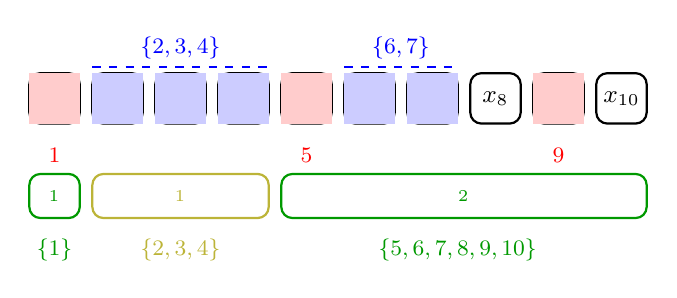
\begin{tikzpicture}[scale=0.8, every node/.style={align=center, font=\small}]
        % Draw the sequence of tokens
        \foreach \i in {1, 2, 3, 4, 5, 6, 7, 8, 9, 10} {
            \draw[rounded corners, thick] (\i, 0) rectangle (\i+0.8, 0.8) node[pos=.5] {$x_{\i}$};
        }

        % Highlight previously sampled tokens (M_<i)
        \foreach \i in {2, 3, 4, 6, 7} {
            \fill[blue!20] (\i, 0) rectangle (\i+0.8, 0.8);
        }

        % Highlight contiguous segments in M_<i
        \draw[thick, dashed, blue] (2, 0.9) -- (4.8, 0.9); % First segment: {2, 3, 4}
        \node[blue] at (3.4, 1.2) {\footnotesize $\{2, 3, 4\}$};

        \draw[thick, dashed, blue] (6, 0.9) -- (7.8, 0.9); % Second segment: {6, 7}
        \node[blue] at (6.9, 1.2) {\footnotesize $\{6, 7\}$};

        % Highlight current sampled tokens (M_i)
        \foreach \i in {1, 5, 9} {
            \fill[red!20] (\i, 0) rectangle (\i+0.8, 0.8);
        }

        % Label current tokens
        \node[red] at (1.4, -0.5) {\footnotesize $1$};
        \node[red] at (5.4, -0.5) {\footnotesize $5$};
        \node[red] at (9.4, -0.5) {\footnotesize $9$};

        % Draw intervals
        \draw[thick, green!60!black, rounded corners] (1, -1.5) rectangle (1.8, -0.8) node[pos=.5] {\small $\gI_1$};
        \node[green!60!black] at (1.4, -2) {\footnotesize $\{1\}$};

        \draw[thick, green!60!black, rounded corners] (5, -1.5) rectangle (10.8, -0.8) node[pos=.5] {\small $\gI_2$};
        \node[green!60!black] at (7.8, -2) {\footnotesize $\{5, 6, 7, 8, 9, 10\}$};

        \draw[thick, yellow!70!black, rounded corners] (2, -1.5) rectangle (4.8, -0.8) node[pos=.5] {\small $\gS_1$};
        \node[yellow!70!black] at (3.4, -2) {\footnotesize $\{2,3,4\}$};
    \end{tikzpicture}
    \caption{Illustration of the example for computing dependencies in the $n$-gram setting. Tokens $x_2, x_3, x_4, x_6, x_7$ (blue) represent the previously sampled location set $\gM_{<i}$, forming two contiguous segments: $\{2, 3, 4\}$ and $\{6, 7\}$. The current sampled locations $x_1, x_5, x_9$ (red) overlap with disjoint intervals $\gI_1 = \{1\}$ and $\gI_2 = \{5, 6, 7, 8, 9, 10\}$. The number of dependencies is computed as $\DEP_n(\gM_i, \gM_{<i}) = |\gM_i| - \text{(number of overlapping intervals)} = 3 - 2 = 1$.}
    \label{fig:dependencies}
\end{figure}


\noindent This example demonstrates how dependencies are computed, highlighting the interaction between previously sampled locations and the current reverse step. Such formalization is critical for understanding the efficiency and accuracy of discrete diffusion processes.

Finally, we extend this concept to define the total number of dependencies across an entire reverse process:

\begin{definition}[Number of Dependencies in a Reverse Process]
    Consider a reverse process $\tau = (\gM_1, \gM_2, \dots, \gM_N)$. Under the $n$-gram setting, the total number of dependencies in the process is defined as the sum of the dependencies across all steps:
    \[
    \DEP_n(\tau) = \sum_{i=1}^N \DEP_n(\gM_i, \gM_{<i}).
    \]
\end{definition}

Using the definition of $\DEP_n(\tau)$, we can bound the KL divergence between the distribution of sequences sampled under an instance of the reverse process and the ground-truth distribution in the $n$-gram setting.

\begin{lemma}[KL Divergence Upper Bound for the Instance of Reverse Process]
\label{lemma:kl_upper_ins_rev}
    Let $q$ denote the data distribution for sequences of length $L$, and let $p$ denote the distribution of sequences of length $L$ generated by reverse model $p_\theta$ via the reverse process $\tau$. Under \cref{ass:perfect_learning}, the following upper bound holds:
    \[
    \DKL{q}{p(\cdot|\tau)} \leq \DEP_n(\tau) \log |\gV|+L\eps_\mathrm{learning},
    \]
    where $\gV$ denote the vocabulary.
\end{lemma}

\begin{proof}
    Using \cref{lemma:kl_decomp_rev}, we have:
    $$\DKL{q}{p_\tau} = \sum_{i=1}^N \mathbb{E}_{\Tilde{\vx}_{<i}}\DKL{q(\Tilde{\vx}_i | \Tilde{\vx}_{<i})}{p_\tau(\Tilde{\vx}_i | \Tilde{\vx}_{<i})}.$$
    For each time step $t_i$:
    $$\mathbb{E}_{\Tilde{\vx}_{<i}}\DKL{q(\Tilde{\vx}_i | \Tilde{\vx}_{<i})}{p_\tau(\Tilde{\vx}_i | \Tilde{\vx}_{<i})}=\mathbb{E}_{\Tilde{\vx}_{<i}}\sum_{\Tilde{\vx}_i\in\gV^{|\gM_i|}}q(\Tilde{\vx}_i | \Tilde{\vx}_{<i})\log\frac{q(\Tilde{\vx}_i | \Tilde{\vx}_{<i})}{p_\tau(\Tilde{\vx}_i | \Tilde{\vx}_{<i})}.$$
    Given $\gM_i$ and $\gM_{<i}$, the tokens $\Tilde{\vx}_i$ at step $t_i$ can be partitioned into independently sampled token sets $\Tilde{\vx}_i^{(1)},\cdots,\Tilde{\vx}_i^{(m)}$ with $k_j$ denoting the size of each token set: 
    $$k_j=|\Tilde{\vx}_i^{(j)}|,\ j\in[m],\quad m=|\gM_i|-\DEP_n(\gM_i,\gM_{<i}).$$
    Using the independence, for each $\Tilde{\vx}_{<i}$, we can decompose the sum into:
    \begin{align*}
    \sum_{\Tilde{\vx}_i\in\gV^{|\gM_i|}}q(\Tilde{\vx}_i | \Tilde{\vx}_{<i})\log\frac{q(\Tilde{\vx}_i | \Tilde{\vx}_{<i})}{p_\tau(\Tilde{\vx}_i | \Tilde{\vx}_{<i})}&=\sum_{j=1}^m\sum_{\Tilde{\vx}_i^{(j)}\in\gV^{k_j}}q(\Tilde{\vx}_i^{(j)} | \Tilde{\vx}_{<i})\log\frac{q(\Tilde{\vx}_i^{(j)} | \Tilde{\vx}_{<i})}{p_\tau(\Tilde{\vx}_i^{(j)} | \Tilde{\vx}_{<i})}\\
    &=\sum_{j=1}^m\DKL{q(\Tilde{\vx}_i^{(j)} | \Tilde{\vx}_{<i})}{p_\tau(\Tilde{\vx}_i^{(j)} | \Tilde{\vx}_{<i}}.
    \end{align*}
    Under \cref{ass:perfect_learning}, the KL divergence between $q$ and $p_\theta$ is bounded by:
    $$\DKL{q_{0|t}(x_0^i \mid \vx_t)}{p_\mathbf{\theta}(x_0^i \mid \vx_t)} < \epsilon_\text{learning}, \quad \forall\ t \text{ and } \vx_t.$$
    By \cref{lemma:kl_mul_token_sample}, we know that:
    $$\DKL{q(\Tilde{\vx}_i^{(j)} | \Tilde{\vx}_{<i})}{p_\tau(\Tilde{\vx}_i^{(j)} | \Tilde{\vx}_{<i}}\leq (k_j-1)\log|\gV|+k_j\eps_\mathrm{learning}.$$
    Substituting back:
    $$\sum_{\Tilde{\vx}_i\in\gV^{|\gM_i|}}q(\Tilde{\vx}_i | \Tilde{\vx}_{<i})\log\frac{q(\Tilde{\vx}_i | \Tilde{\vx}_{<i})}{p_\tau(\Tilde{\vx}_i | \Tilde{\vx}_{<i})}\leq\sum_{j=1}^m(k_j-1)\log|\gV|+k_j\eps_\mathrm{learning}.$$
    Using the fact that
    $$\sum_{j=1}^m(k_j-1)=|\gM_i|-m=\DEP_n(\gM_i,\gM_{<i}),\quad \sum_{j=1}^mk_j=|\gM_i|$$
    we can obtain:
    $$\mathbb{E}_{\Tilde{\vx}_{<i}}\DKL{q(\Tilde{\vx}_i | \Tilde{\vx}_{<i})}{p_\tau(\Tilde{\vx}_i | \Tilde{\vx}_{<i})}\leq \DEP_n(\gM_i,\gM_{<i})\log|\gV|+|\gM_i|\eps_\mathrm{learning}.$$
    Thus, combined with the definition of $\DEP_n(\tau)$ and $p_\tau=p(\cdot|\tau)$, we can draw the final conclusion:
    \begin{align*}
        \DKL{q}{p(\cdot|\tau)} &\leq \sum_{i=1}^N\left(\DEP_n(\gM_i,\gM_{<i})\log|\gV|+|\gM_i|\eps_\mathrm{learning}\right)\\
        &=\DEP_n(\tau) \log |\gV|+L\eps_\mathrm{learning}.
    \end{align*}
    %In other words:
    %$$\DKL{q}{p(\cdot|\tau)} = \sum_{i=1}^N \DKL{q(\Tilde{\vx}_i | \Tilde{\vx}_{<i})}{p_\tau(\Tilde{\vx}_i | \Tilde{\vx}_{<i})}.$$
\end{proof}

The above Lemma directly leads to the bound for the KL divergence between the distribution of sequences generated by the reverse model with a given masking schedule and the ground-truth distribution in the $n$-gram setting.

\begin{lemma}[KL Divergence Upper Bound for a Masking Schedule]
\label{lemma:kl_bound_mask}
    Let $q$ denote the data distribution over sequences of length $L$, and let $p$ denote the distribution over sequences of length $L$ generated by the reverse model $p_\theta$ with masking schedule $\alpha_t$ and $N$ reverse steps. Under \cref{ass:perfect_learning}, the KL divergence between $q$ and $p$ satisfies the following upper bound:
    \[
    \DKL{q}{p} \leq \log |\gV| \sum_{i=1}^N \E_{\tau\sim\PROC(L, \alpha_t, N)} \DEP_n(\gM_i, \gM_{<i})+L\eps_\mathrm{learning}.
    \]
\end{lemma}

\begin{proof}
    By \cref{lemma:kl_upper_mask}, we can obtain:
    $$\DKL{q}{p} \leq \mathbb{E}_{\tau \sim \PROC(\alpha_t, N, L)} \DKL{q}{p(\cdot | \tau)}.$$
    Applying \cref{lemma:kl_upper_ins_rev} to the instances of reverse process, we can conclude that:
    \begin{align*}
    \DKL{q}{p} &\leq \mathbb{E}_{\tau \sim \PROC(\alpha_t, N,L)}\sum_{i=1}^N\DEP_n(\gM_i,\gM_{<i})\log|\gV|+L\eps_\mathrm{learning}\\
    &=\log |\gV| \sum_{i=1}^N \E_{\tau\sim\PROC(L, \alpha_t, N)} \DEP_n(\gM_i, \gM_{<i})+L\eps_\mathrm{learning}.
    \end{align*}
\end{proof}

For the final estimation, we need to derive an upper bound for the expected number of dependencies at each reverse step. First, we use Chernoff Bound to control the number of separators and new locations at each reverse step for a given masking schedule.

\begin{lemma}[Bounds on Separator and New Location Count at Each Reverse Step]
\label{lemma:bound_sep_new_rev}
    Given a sequence of length $L$, a masking schedule $\alpha_t$, and $N$ reverse steps. Assume that $L$ is divisible by $n-1$. Given the time step $t_i = \frac{N-i}{N}$, let $\NEW$ denote the number of locations sampled at step $t_i$, and $\SEP_n$ denote the number of separators in the previously sampled locations. Under the $n$-gram setting, the following bounds hold for $\NEW$ and $\SEP_n$:
    \begin{align*}
        \Pr\left(\SEP_n\leq \frac{Lp_i^{n-1}}{2(n-1)}\right)&\leq e^{-\frac{Lp_i^{n-1}}{8(n-1)}},\\
        \Pr\left(\NEW\geq 2L\delta_i\right)&\leq e^{-\frac{L\delta_i}{3}},
    \end{align*}
    where $p_i = \alpha_{t_{i-1}}$ and $\delta_i = \alpha_{t_i} - \alpha_{t_{i-1}}$.
\end{lemma}

\begin{proof}
Given a masking schedule $\alpha_t$, using the expression of true reverse process in \cref{eq:rev_proc} and $\alpha_1=0$, we can compute the probability $p^{(i)}$ of a token being sampled at time step $t_i$ to be:
$$p^{(i)}=\frac{\alpha_{t_i}-\alpha_{t_{i-1}}}{1-\alpha_{t_{i-1}}}\cdot\prod_{j=1}^{i-1}\frac{1-\alpha_{t_j}}{1-\alpha_{t_{j-1}}}=\alpha_{t_i} - \alpha_{t_{i-1}}=\delta_i.$$
Therefore, $\delta_i$ is the probability of a location being sampled at time step $t_i$. Summing up $\delta_i$, we can know that $p_i=\sum_{j=1}^{i-1}\delta_j$ is the probability of a location being sampled prior to time step $t_i$.

To derive a bound for $\SEP_n$, we partition the sequence into $\frac{L}{n-1}$ intervals, each of length $n-1$. For a given interval, the probability that all locations within the interval have been sampled prior to step $t_i$ is $p_i^{n-1}$. Define $X_j=1$ if the locations in the $j$-th interval have been sampled prior to $t_i$, and $X_j=0$ otherwise. The random variables $X_1,X_2,\cdots,X_{\frac{L}{n-1}}$ are independent and satisfy the following expectation:
$$\mathbb{E}_{\tau \sim \PROC(L, \alpha_t, N)}\sum_{j=1}^{\frac{L}{n-1}}X_j=\frac{Lp_i^{n-1}}{n-1}.$$
By the definition of $\SEP_n$, we know that:
$$\SEP_n\geq\sum_{j=1}^{\frac{L}{n-1}}X_j.$$
Applying \cref{lemma:chernoff} to the sum of $X_j$, we derive:
$$\Pr\left(\SEP_n\leq \frac{Lp_i^{n-1}}{2(n-1)}\right)\leq \Pr\left(\sum_{j=1}^{\frac{L}{n-1}}X_j\leq \frac{Lp_i^{n-1}}{2(n-1)}\right)\leq e^{-\frac{Lp_i^{n-1}}{8(n-1)}}.$$

Next, we consider the bound for $\NEW$. Given that the sequence contains $L$ locations and the probability of sampling any specific location at step $t_i$ is $\delta_i$, the expected number of new locations sampled at $t_i$ is given by:
$$\mathbb{E}_{\tau \sim \PROC(L, \alpha_t, N)}\NEW=L\delta_i.$$
Since the sampling of each location occurs independently, applying \cref{lemma:chernoff}, we have:
$$\Pr\left(\NEW\geq 2L\delta_i\right)\leq e^{-\frac{L\delta_i}{3}}.$$
\end{proof}

Using the above lemma, we can divide the estimation for the number of dependencies into three cases, and derive the bound case by case. This is achieved by using a variety of means and careful estimations.

\begin{lemma}[Upper Bound for the Expectation of Dependencies at Each Reverse Step]
\label{lemma:bound_dep_rev}
    Given a sequence of length $L$, a masking schedule $\alpha_t$, and $N$ reverse steps. Assume $L\delta_i>1$, then the expected number of dependencies at time step $t_i = \frac{N-i}{N}$ satisfies:
    \[
    \mathbb{E}_{\tau \sim \PROC(L, \alpha_t, N)} \DEP_n(\gM_i, \gM_{<i}) \leq \frac{9}{3+L\delta_i}+\frac{C(n-1)L\delta_i^2}{p_i^{n-1}},
    \]
    where $p_i = \alpha_{t_{i-1}}$, $\delta_i = \alpha_{t_i} - \alpha_{t_{i-1}}$, and $C$ is a constant.
\end{lemma}

\begin{proof}
By \cref{lemma:bound_sep_new_rev}, at step $t_i$, the following bounds hold:
\begin{align*}
        \Pr\left(\SEP_n\leq \frac{Lp_i^{n-1}}{2(n-1)}\right)&\leq e^{-\frac{Lp_i^{n-1}}{8(n-1)}},\\
        \Pr\left(\NEW\geq 2L\delta_i\right)&\leq e^{-\frac{L\delta_i}{3}}.
\end{align*}
Since $\DEP_n(\gM_i, \gM_{<i})\geq 0$, its expectation can be decomposed into three components:
\begin{align*}
    \mathbb{E}_{\tau \sim \PROC(L, \alpha_t, N)} \DEP_n(\gM_i, \gM_{<i})&=\Pr\left(\NEW\geq 2L\delta_i\right)\cdot \mathbb{E}_{\substack{\tau \sim \PROC(L, \alpha_t, N)\\ \NEW\geq 2L\delta_i}} \DEP_n(\gM_i, \gM_{<i})&\textbf{(Case 1)}\\
    &+\Pr\left(\SEP_n\leq \frac{Lp_i^{n-1}}{2(n-1)},\ \NEW< 2L\delta_i\right)\cdot \\
    &\qquad\mathbb{E}_{\substack{\tau \sim \PROC(L, \alpha_t, N)\\ \SEP_n\leq \frac{Lp_i^{n-1}}{2(n-1)}\\ \NEW< 2L\delta_i}} \DEP_n(\gM_i, \gM_{<i}) &\textbf{(Case 2)}\\
    &+\Pr\left(\SEP_n>\frac{Lp_i^{n-1}}{2(n-1)},\ \NEW< 2L\delta_i\right)\cdot \\
    &\qquad\mathbb{E}_{\substack{\tau \sim \PROC(L, \alpha_t, N)\\ \SEP_n>\frac{Lp_i^{n-1}}{2(n-1)}\\ \NEW<2L\delta_i}} \DEP_n(\gM_i, \gM_{<i})&\textbf{(Case 3)}
\end{align*}
We estimate these three cases separately.

\textbf{Case 1:} $\NEW\geq 2L\delta_i$.

By the definitions of $\DEP_n(\gM_i, \gM_{<i})$ and $\NEW$, we have:
$$\DEP_n(\gM_i, \gM_{<i})\leq |\gM_i|=\NEW.$$
Substituting this into the estimation, we obtain:
$$\Pr\left(\NEW\geq 2L\delta_i\right)\cdot \mathbb{E}_{\substack{\tau \sim \PROC(L, \alpha_t, N)\\ \NEW\geq 2L\delta_i}} \DEP_n(\gM_i, \gM_{<i})\leq \Pr\left(\NEW\geq 2L\delta_i\right)\cdot \mathbb{E}_{\substack{\tau \sim \PROC(L, \alpha_t, N)\\ \NEW\geq 2L\delta_i}} \NEW$$
Since $\DEP_n(\gM_i, \gM_{<i})\geq 0$, the expectation can be expressed as an integral of the tail probability:
$$\mathbb{E}_{\substack{\tau \sim \PROC(L, \alpha_t, N)\\ \NEW\geq 2L\delta_i}} \NEW=\int_{2L\delta_i}^{+\infty} \Pr\left(\NEW\geq x\mid\NEW\geq 2L\delta_i\right)\dd x.$$
It directly follows that:
\begin{align*}
    \Pr\left(\NEW\geq 2L\delta_i\right)\cdot \mathbb{E}_{\substack{\tau \sim \PROC(L, \alpha_t, N)\\ \NEW\geq 2L\delta_i}} \NEW &=\Pr\left(\NEW\geq 2L\delta_i\right)\cdot \int_{2L\delta_i}^{+\infty} \Pr\left(\NEW\geq x\mid\NEW\geq 2L\delta_i\right)\dd x\\
    &=\int_{2L\delta_i}^{+\infty} \Pr\left(\NEW\geq x\mid\NEW\geq 2L\delta_i\right)\Pr\left(\NEW\geq 2L\delta_i\right)\dd x\\
    &=\int_{2L\delta_i}^{+\infty}\Pr\left(\NEW\geq x\right)\dd x.
\end{align*}
Using the same trick as \cref{lemma:bound_sep_new_rev}, applying \cref{lemma:chernoff}, we can derive the bound for probability $\Pr\left(\NEW\geq x\right)$ as:
$$\Pr\left(\NEW\geq x\right)\leq e^{-\frac{(x-L\delta_i)^2}{x+L\delta_i}}.$$
Note that $\NEW\leq L$, we only need to consider $2\delta_i\leq 1$. In this case, we have:
\begin{align*}
    \int_{2L\delta_i}^{+\infty}\Pr\left(\NEW\geq x\right)\dd x \leq \int_{2L\delta_i}^{L}e^{-\frac{(x-L\delta_i)^2}{x+L\delta_i}}\dd x
\end{align*}
Let $y=x-L\delta_i\in[L\delta_i,L(1-\delta_i)]$, the integral can be rewritten as:
$$\int_{2L\delta_i}^{+\infty}\Pr\left(\NEW\geq x\right)\dd x \leq \int_{L\delta_i}^{L(1-\delta_i)}e^{-\frac{y^2}{y+2L\delta_i}}\dd y.$$
Observe that $y+2L\delta_i\leq 3y$, we can obtain:
$$\int_{2L\delta_i}^{+\infty}\Pr\left(\NEW\geq x\right)\dd x \leq \int_{L\delta_i}^{L(1-\delta_i)}e^{-\frac{y^2}{3y}}\dd y =3\left(e^{-\frac{L\delta_i}{3}}-e^{-\frac{L(1-\delta_i)}{3}}\right)=3e^{-\frac{L\delta_i}{3}}\left(1-e^{-\frac{L(1-2\delta_i)}{3}}\right).$$
Using the fact that $e^{-x}\leq\frac{1}{1+x}$ for $x\geq 0$, we have the upper bound:
$$3e^{-\frac{L\delta_i}{3}}\left(1-e^{-\frac{L(1-2\delta_i)}{3}}\right)\leq 3e^{-\frac{L\delta_i}{3}}\leq \frac{9}{3+L\delta_i}.$$
Combining the above results, we know that:
$$\Pr\left(\NEW\geq 2L\delta_i\right)\cdot \mathbb{E}_{\substack{\tau \sim \PROC(L, \alpha_t, N)\\ \NEW\geq 2L\delta_i}} \DEP_n(\gM_i, \gM_{<i})\leq \frac{9}{3+L\delta_i}.$$

\textbf{Case 2:} $\SEP_n\leq \frac{Lp_i^{n-1}}{2(n-1)}$ and $ \NEW<2L\delta_i$.

Similar to Case 1, we have:
$$\DEP_n(\gM_i, \gM_{<i})\leq\NEW<2L\delta_i,$$
so the expectation also follows:
$$\mathbb{E}_{\substack{\tau \sim \PROC(L, \alpha_t, N)\\ \SEP_n\leq \frac{Lp_i^{n-1}}{2(n-1)}\\ \NEW< 2L\delta_i}} \DEP_n(\gM_i, \gM_{<i})< 2L\delta_i.$$
Using the probability bound, it follows that:
$$\Pr\left(\SEP_n\leq \frac{Lp_i^{n-1}}{2(n-1)},\ \NEW< 2L\delta_i\right)\leq\Pr\left(\SEP_n\leq \frac{Lp_i^{n-1}}{2(n-1)}\right)\leq e^{-\frac{Lp_i^{n-1}}{8(n-1)}}.$$
Since $e^{-x}\leq\frac{1}{1+x}$ for $x\geq 0$:
$$e^{-\frac{Lp_i^{n-1}}{8(n-1)}}\leq\frac{8(n-1)}{Lp_i^{n-1}+8(n-1)}.$$
Combining these results, we obtain:
$$\Pr\left(\SEP_n\leq \frac{Lp_i^{n-1}}{2(n-1)},\ \NEW< 2L\delta_i\right)\cdot\mathbb{E}_{\substack{\tau \sim \PROC(L, \alpha_t, N)\\ \SEP_n\leq \frac{Lp_i^{n-1}}{2(n-1)}\\ \NEW< 2L\delta_i}} \DEP_n(\gM_i, \gM_{<i})\leq \frac{16(n-1)L\delta_i}{Lp_i^{n-1}+8(n-1)}.$$

\textbf{Case 3:} $\SEP_n>\frac{Lp_i^{n-1}}{2(n-1)}$ and $ \NEW<2L\delta_i$.

Apparently, we have:
$$\Pr\left(\SEP_n>\frac{Lp_i^{n-1}}{2(n-1)},\ \NEW< 2L\delta_i\right)\leq 1.$$
Given $a,b$, let $\mathbb{E}_{a,b}\DEP_n(\gM_i, \gM_{<i})$ denote the expectation of $\DEP_n(\gM_i, \gM_{<i})$ under the condition of $\SEP_n=a$ and $ \NEW=b$. In other words:
$$\mathbb{E}_{a,b}\DEP_n(\gM_i, \gM_{<i})=\mathbb{E}_{\substack{\tau \sim \PROC(L, \alpha_t, N)\\ \SEP_n=a\\ \NEW=b}} \DEP_n(\gM_i, \gM_{<i}).$$
Since all the locations are sampled independently, and $\DEP_n(\gM_i, \gM_{<i})$ depends only on the relative positions of separators in $\gM_{<i}$ and the new locations in $\gM_i$, the expectation $\mathbb{E}_{a,b}\DEP_n(\gM_i, \gM_{<i})$ only depends on the ordering of separators and new locations.

Assume $x_1,\cdots,x_{a+b}$ are $a+b$ positions (not locations) in order. We can regard the process of ordering separators and new locations as the process of choosing $b$ positions randomly from $x_j$. For $1\leq j\leq a+b-1$, define $X_j=1$ if $x_j$ and $x_{j+1}$ are both new locations, and $X_j=0$ otherwise. By the definition of $\DEP_n(\gM_i, \gM_{<i})$, we can obtain:
$$\DEP_n(\gM_i, \gM_{<i})=\sum_{j=1}^{a+b-1}X_j.$$
Since the $b$ new locations are chosen randomly, the probability of $X_j=1$ can be calculated as:
$$\Pr(X_j=1)=\frac{C_{a+b-2}^{b-2}}{C_{a+b}^{b}}=\frac{b(b-1)}{(a+b)(a+b-1)}.$$
Therefore, the expectation of $X_j$ is:
$$\mathbb{E}X_j=\frac{b(b-1)}{(a+b)(a+b-1)}.$$
Summing up, we have:
$$\mathbb{E}_{a,b}\DEP_n(\gM_i, \gM_{<i})=\mathbb{E}\sum_{j=1}^{a+b-1}X_j=(a+b-1)\mathbb{E}X_1=\frac{b(b-1)}{a+b}.$$
Since $a>\frac{Lp_i^{n-1}}{2(n-1)}$ and $b<2L\delta_i$, we can derive the upper bound for any $a,b$:
$$\frac{b(b-1)}{a+b}\leq \frac{b(b-1)}{\frac{Lp_i^{n-1}}{2(n-1)}+b} \leq\frac{2L\delta_i(2L\delta_i-1)}{\frac{Lp_i^{n-1}}{2(n-1)}+2L\delta_i}\leq \frac{8(n-1)L\delta_i^2}{p_i^{n-1}+4(n-1)\delta_i}.$$
Since this holds for all $a$ and $b$, we can obtain:
\begin{align*}
    &\quad\Pr\left(\SEP_n>\frac{Lp_i^{n-1}}{2(n-1)},\ \NEW< 2L\delta_i\right)\cdot\mathbb{E}_{\substack{\tau \sim \PROC(L, \alpha_t, N)\\ \SEP_n>\frac{Lp_i^{n-1}}{2(n-1)}\\ \NEW<2L\delta_i}} \DEP_n(\gM_i, \gM_{<i})\\
    &\leq \mathbb{E}_{\substack{\tau \sim \PROC(L, \alpha_t, N)\\ \SEP_n>\frac{Lp_i^{n-1}}{2(n-1)}\\ \NEW<2L\delta_i}} \DEP_n(\gM_i, \gM_{<i})\\
    &=\sum_{a>\frac{Lp_i^{n-1}}{2(n-1)},\ b<2L\delta_i}\Pr(\SEP_n=a, \NEW=b)\cdot\mathbb{E}_{a,b}\DEP_n(\gM_i, \gM_{<i})\\
    &\leq \frac{8(n-1)L\delta_i^2}{p_i^{n-1}+4(n-1)\delta_i}.
\end{align*}

\textbf{Summarize the above proof:}

Combining the above three cases, we can obtain:
$$\mathbb{E}_{\tau \sim \PROC(L, \alpha_t, N)} \DEP_n(\gM_i, \gM_{<i}) \leq \frac{9}{3+L\delta_i}+\frac{16(n-1)L\delta_i}{Lp_i^{n-1}+8(n-1)}+\frac{8(n-1)L\delta_i^2}{p_i^{n-1}+4(n-1)\delta_i}.$$
If we have the assumption $L\delta_i\geq 1$, it is easy to find that:
\begin{align*}
    \mathbb{E}_{\tau \sim \PROC(L, \alpha_t, N)} \DEP_n(\gM_i, \gM_{<i}) &\leq \frac{9}{3+L\delta_i}+\frac{16(n-1)\delta_i}{p_i^{n-1}}+\frac{8(n-1)L\delta_i^2}{p_i^{n-1}}\\
    &\leq \frac{9}{3+L\delta_i}+\frac{16(n-1)L\delta_i^2}{p_i^{n-1}}+\frac{8(n-1)L\delta_i^2}{p_i^{n-1}}\\
    &\leq \frac{9}{3+L\delta_i}+\frac{C(n-1)L\delta_i^2}{p_i^{n-1}}.
\end{align*}
Where $C=24$ is a constant.

\end{proof}

Finally, we can derive the upper bound for the KL divergence between the distribution of sequences generated by the
reverse model and the ground-truth distribution in the n-gram setting.

\begin{lemma}[Efficient Sampling with Small KL Divergence]
\label{lemma:effi_kl_bound}
    Let $q$ denote the data distribution over sequences of length $L$, and let $p$ denote the distribution over sequences of length $L$ generated by the reverse model $p_\theta$ with a masking schedule $\alpha_t$ and $N$ reverse steps. Assume that $p_\theta$ satisfies \cref{ass:perfect_learning}. For any $\epsilon > 0$, there exists a masking schedule $\alpha_t$ such that, for $L\geq \frac{3C(n-1)}{\eps^{n+\frac{1}{2}}}$, with $N = O\left(\frac{n-1}{\eps^{n}}\right)$ sampling steps, the KL divergence between $q$ and $p$ satisfies:
    $$\frac{\DKL{q}{p}}{L\log|\gV|} \leq 4\eps +\frac{\eps_\mathrm{learning}}{\log|\gV|}.$$
\end{lemma}

\begin{proof}
    By \cref{lemma:kl_bound_mask}, we know that:
    $$\DKL{q}{p} \leq \log |\gV| \sum_{i=1}^N \E_{\tau\sim\PROC(L, \alpha_t, N)} \DEP_n(\gM_i, \gM_{<i})+L\eps_\mathrm{learning}.$$
    Note that at step $t_1$, the reverse process can be bounded using \cref{lemma:kl_mul_token_sample}. By reviewing our proof process, it is easy to see that we can substitute $\DEP_n(\gM_1, \gM_{<1})$ for $(|\gM_1|-1)\log |\gV|$, where $\gV$ stands for the vocabulary. By the definition of $\delta_i$, we know that:
    $$\E_{\tau\sim\PROC(L, \alpha_t, N)} (|\gM_1|-1)\log |\gV|=(\delta_1L-1)\log |\gV|.$$
    Applying \cref{lemma:bound_dep_rev} to $\DEP_n(\gM_i, \gM_{<i})$, if $L\delta_i\geq 1$, we can obtain:
    $$\DKL{q}{p}\leq \delta_1\log |\gV|+\log |\gV| \sum_{i=2}^N\left(\frac{9}{3+L\delta_i}+\frac{C(n-1)L\delta_i^2}{p_i^{n-1}}\right)+L\eps_\mathrm{learning}.$$
    By the definition of $p_i$, we know that $p_2=\delta_1$. For any small $\eps>0$, consider the following masking schedule:
    %$$\delta_1=\frac{\eps}{\log |\gV|},\quad \delta_i=\delta=\frac{\eps^n}{C(n-1)(\log|\gV|)^n},\quad p_i=\delta_1+(i-2)\delta,\quad\forall i\geq 2.$$
    $$\delta_1=\eps,\quad \delta_i=\delta=\frac{\eps^n}{C(n-1)},\quad p_i=\delta_1+(i-2)\delta,\quad\forall i\geq 2.$$
    Then, for $L\geq \frac{1}{\delta}$, the KL divergence can be bounded by:
    \begin{align*}
        \frac{\DKL{q}{p}}{L\log|\gV|}&\leq \eps+\frac{9(N-1)}{L(3+L\delta)}+\sum_{i=2}^N \frac{C(n-1)\delta^2}{p_i^{n-1}}+\frac{\eps_\mathrm{learning}}{\log|\gV|}\\
        &=\eps+\frac{9(1-\delta_1)}{L\delta(3+L\delta)}+\frac{C(n-1)\delta^2}{\delta_1^{n-1}}+\sum_{i=1}^{N-2} \frac{C(n-1)\delta^2}{(\delta_1+i\delta)^{n-1}}+\frac{\eps_\mathrm{learning}}{\log|\gV|}.\\
        &\leq \eps+\frac{9}{L\delta(3+L\delta)}+\frac{C(n-1)\delta^2}{\delta_1^{n-1}}+\sum_{i=1}^{N-2} \frac{C(n-1)\delta^2}{(\delta_1+i\delta)^{n}}+\frac{\eps_\mathrm{learning}}{\log|\gV|}.
    \end{align*}
    By simple calculations, we know that:
    $$\frac{9}{L\delta(3+L\delta)}\leq \eps,\quad \text{if }L\geq \frac{3}{\delta\eps^{\frac{1}{2}}}.$$
    It is clear that $\delta\leq 1$, so:
    $$\frac{C(n-1)\delta^2}{\delta_1^{n-1}}\leq \eps\delta\leq\eps.$$
    Since $x^{-n}$ is convex on $[0,+\infty)$, the accumulation can be bounded by:
    \begin{align*}
        \sum_{i=1}^{N-2} \frac{C(n-1)\delta^2}{(\delta_1+i\delta)^n}&=C(n-1)\delta^{2-n}\sum_{i=1}^{N-2}\frac{1}{(\frac{\delta_1}{\delta}+i)^n}\\
        &\leq C(n-1)\delta^{2-n}\sum_{i=1}^{N-2}\int_{x=0}^{+\infty}\frac{1}{(\frac{\delta_1}{\delta}+x)^n\dd x}\\
        &=C(n-1)\delta^{2-n}\cdot\frac{1}{n-1}\left(\frac{\delta}{\delta_1}\right)^{n-1}\\
        &=\frac{C\delta}{\delta_1^{n-1}}\\
        &\leq\eps.
    \end{align*}
    Combining the above, we have:
    $$\frac{\DKL{q}{p}}{L\log|\gV|}\leq 4\eps+\frac{\eps_\mathrm{learning}}{\log|\gV|}.$$
    Meanwhile, the time step is limited by:
    $$N=1+\frac{1-\delta_1}{\delta}=O\left(\frac{n-1}{\eps^n}\right),$$
    and the lower bound for $L$:
    $$L\geq \frac{3}{\delta\eps^{\frac{1}{2}}}=\frac{3C(n-1)}{\eps^{n+\frac{1}{2}}}.$$

\end{proof}

Combining the above lemmas, we can prove \cref{thm:acceleration_ngram} by breaking the expression of $\log\PPL(p)$ into two parts.

\begin{theorem}[$\PPL$ Bounds for $n$-Gram Language Generation]
    For any $n$-gram language $q$ and any $\epsilon > 0$, let $p_\mathsf{\theta}$ denote the reverse model and $L$ denote the sequence length. The distribution over sequences generated by $p_\mathsf{\theta}$ is denoted as $p$. For any $L>O\big( \frac{n-1}{\epsilon^{n+0.5}}\big)$, under \cref{ass:perfect_learning}, there exists a masking schedule $\alpha_t$ such that, with $N = O\big( \frac{n-1}{\epsilon^n}\big)$ sampling steps, the perplexity of the MDM is upper-bounded by:
    $$\log\PPL(p) \leq \log\PPL(q) + \epsilon_\text{learning} + 4\epsilon\log |\gV|.$$
\end{theorem}

\begin{proof}
    By \cref{lemma:effi_kl_bound}, for any $L>O\big( \frac{n-1}{\epsilon^{n+0.5}}\big)$, there exists a masking schedule $\alpha_t$ with $N = O\big( \frac{n-1}{\epsilon^n}\big)$ sampling steps satisfying:
    $$\frac{\DKL{q}{p}}{L\log|\gV|} \leq 4\eps+\frac{\eps_\mathrm{learning}}{\log|\gV|}.$$
    In other words:
    $$\frac{1}{L}\mathbb{E}_{\vx \sim q}
    \log \frac{q(\vx)}{p(\vx)}\leq 4\eps\log|\gV|+\eps_\mathrm{learning}.$$
    By the definition of $\PPL$, we have:
    $$\log\PPL(p) = \mathbb{E}_{\vx \sim q} -\frac{\log p(\vx)}{|\vx|}=\frac{1}{L}\mathbb{E}_{\vx \sim q}\left(-\log q(\vx)+\log\frac{q(\vx)}{p(\vx)}\right).$$
    Note that:
    $$\log\PPL(q) = \mathbb{E}_{\vx \sim q} -\frac{\log q(\vx)}{|\vx|}=\frac{1}{L}\mathbb{E}_{\vx \sim q}-\log q(\vx).$$
    We can obtain:
    $$\log\PPL(p) \leq \log\PPL(q) + \epsilon_\text{learning} + 4\epsilon\log |\gV|.$$
\end{proof}


\section{Proof for \cref{thm:pos_hmm} and \cref{thm:negative}}
\subsection{Proof for \cref{thm:pos_hmm}}
\label{app:proof_hmm_pos}
In this section, we aim to derive the upper bound for the $\SER$ of generated sequences with sufficient reverse steps. First, we argue that, given a making schedule $\alpha_t$, with sufficient steps, the probability of sampling multiple locations in the sequence at the same time can be very low.

\begin{lemma}[Low Probability of Simultaneous Sampling with Sufficient Steps]
\label{lemma:prob_mul_suff}
    Given a sequence of length $L$ and a masking schedule $\alpha_t$. For any $\eps>0$, there exists $N_0$, such that for any $N\geq N_0$, with $N$ reverse steps, the probability $p_\mathrm{mul}$ of sampling multiple locations in the sequence at the same time satisfies:
    $$p_\mathrm{mul}<\eps.$$
\end{lemma}

\begin{proof}
    By \cref{lemma:bound_sep_new_rev}, we know that the probability of a location being sampled at time step $t_i=\frac{N-i}{N}$ is:
    $$\delta_i=\alpha_{t_i}-\alpha_{t_{i-1}}=\alpha_\frac{N-i}{N}-\alpha_\frac{N-i+1}{N}.$$
    Since all the locations are sampled independently, for two distinct locations $i\neq j$ in the sequence, the probability that $i$ and $j$ are sampled simultaneously is:
    $$p_{i,j}=\sum_{i=1}^{N}\delta_i^2.$$
    Summing up $p_{i,j}$, the probability of having two locations a=sampled simultaneously can be bounded by:
    $$p_\mathrm{mul}\leq \frac{L(L-1)}{2}\cdot\sum_{i=1}^{N}\delta_i^2$$
    Since $\alpha_t$ is continuous on $[0,1]$, we know that it is uniformly continuous. Therefore, for any $\eps>0$, there exists $N_0>0$ that satisfies:
    $$|\alpha_x-\alpha_y|<\frac{2\eps}{L(L-1)}, \quad\forall x,y\in [0,1], |x-y|<\frac{1}{N_0}.$$
    In this case, for $N>N_0$, we know that:
    $$|\delta_i|=|\alpha_\frac{N-i}{N}-\alpha_\frac{N-i+1}{N}|<\frac{2\eps}{L(L-1)},\quad\forall i\in [N].$$
    Combining with the fact that $\sum_{i=1}^N\delta_i=1$, we can obtain:
    $$p_\mathrm{mul}\leq \frac{L(L-1)}{2}\cdot\sum_{i=1}^{N}\delta_i\cdot\max_{j\in [N]}\delta_j<\eps.$$
\end{proof}

Next, we consider the $\SER$ increase due to the learning error. Specifically, we only investigate the case where all the locations are sampled at different steps.

\begin{lemma}[Accurate Step-by-Step Generation with Low Learning Error]
\label{lemma:acc_gen}
    Let $q$ denote any HMM, and let $p_\mathsf{\theta}$ represent the reverse model under an arbitrary masking schedule, where $L$ is the sequence length. Let $p$ denote the distribution over sequences generated by $p_\mathsf{\theta}$. Under \cref{ass:perfect_learning} with a learning error $\epsilon_\text{learning} < \frac{\delta}{L},\ \delta>0$, and given an instance of reverse process $\tau=(\gM_1,\gM_2,\cdots,\gM_N)$ with $|\gM_i|\leq 1$, let $p_\mathrm{acc}$ denote the probability of generating a valid sequence. Then $p_\mathrm{acc}$ satisfies:
    $$p_\mathrm{acc}\geq e^{-\delta}.$$
\end{lemma}

\begin{proof}
    Since $|\gM_i|\leq 1$, we only need to consider the steps where one token is sampled. Let $\Tilde{\vx}_t$ denote the previously sampled tokens, and $\Tilde{x}_t$ denote the token sampled at the current step. If $\Tilde{\vx}_t$ is can later form a valid sequence, let $\gX_t$ denote the set of valid choices for $\Tilde{x}_t$. In other words, if $\Tilde{x}_t\in \gX_t$, then the combination of $\Tilde{\vx}_t$ and $\Tilde{x}_t$ is can later form a valid sequence, or more intuitively:
    $$q_{0|t}(\Tilde{x}_t\mid\Tilde{\vx}_t)>0.$$
    Under \cref{ass:perfect_learning}, we know that:
    $$\DKL{q_{0|t}(x_t \mid \Tilde{\vx}_t)}{p_\mathbf{\theta}(x_t \mid \Tilde{\vx}_t)} < \epsilon_\text{learning}.$$
    Since it is assumed that $0\log 0=0$, we have:
    $$\sum_{x_t\in\gX_t}q_{0|t}(x_t \mid \Tilde{\vx}_t)\log\frac{q_{0|t}(x_t \mid \Tilde{\vx}_t)}{p_\theta(x_t \mid \Tilde{\vx}_t)}<\eps_\text{learning}.$$
    Equivalently, we have:
    $$-\eps_\text{learning}<\sum_{x_t\in\gX_t}q_{0|t}(x_t \mid \Tilde{\vx}_t)\log\frac{p_\theta(x_t \mid \Tilde{\vx}_t)}{q_{0|t}(x_t \mid \Tilde{\vx}_t)}.$$
    Due to the concavity of $\log x$, by Jensen's Inequality, we can obtain:
    $$\sum_{x_t\in\gX_t}q_{0|t}(x_t \mid \Tilde{\vx}_t)\log\frac{p_\theta(x_t \mid \Tilde{\vx}_t)}{q_{0|t}(x_t \mid \Tilde{\vx}_t)}\leq \log\left(\sum_{x_t\in\gX_t}q_{0|t}(x_t \mid \Tilde{\vx}_t)\cdot \frac{p_\theta(x_t \mid \Tilde{\vx}_t)}{q_{0|t}(x_t \mid \Tilde{\vx}_t)}\right) =\log\sum_{x_t\in\gX_t}p_\theta(x_t \mid \Tilde{\vx}_t).$$
    Therefore, the probability that each step remains valid satisfies:
    $$\sum_{x_t\in\gX_t}p_\theta(x_t \mid \Tilde{\vx}_t)\geq e^{-\eps_\text{learning}}\geq e^{-\frac{\delta}{L}}.$$
    Since there are $L$ locations in the sequence, the probability of generating a valid sequence is bounded by:
    $$p_\mathrm{acc}\geq (e^{-\frac{\delta}{L}})^L=e^{-\delta}.$$
\end{proof}

Combining the above lemmas, we can derive the upper bound of $\SER$ by taking sufficient reverse steps and small learning error.

\begin{theorem}[Accurate Generation of HMM with Sufficient Steps]
    Let $q$ denote any HMM, and let $p_\mathsf{\theta}$ represent the reverse model under an arbitrary masking schedule, where $L$ is the sequence length. Let $p$ denote the distribution over sequences generated by $p_\mathsf{\theta}$. Under \cref{ass:perfect_learning} with a learning error $\epsilon_\text{learning} < O(\frac{\delta}{L})$, and given a sufficient number of reverse steps, the sequence error rate $\operatorname{SER}(p)$ of the generated text satisfies 
    \[
    \operatorname{SER}(p) \leq  \delta.
    \]
\end{theorem}

\begin{proof}
    For $\delta>0$, we know that:
    $$1-\delta<c.$$
    By \cref{lemma:prob_mul_suff}, given the masking schedule $\alpha_t$, there exists $N_0$, for $N>N_0$ and $N$ reverse steps, the probability of sampling multiple locations in the sequence at the same time is bounded by:
    $$p_\mathrm{mul}<1-\frac{1-\delta}{e^{-\delta}}.$$
    In other words, the probability of sampling all the locations at different steps is at least $\frac{1-\delta}{e^{-\delta}}$. By \cref{lemma:acc_gen}, for each reverse process which satisfies that all the locations are sampled at different steps, the probability of generating a valid sequence is lower bounded by:
    $$p_\mathrm{acc}\geq e^{-\delta}.$$
    Therefore, the sequence error rate $\SER$ satisfies:
    $$\SER(p)\leq 1-\frac{1-\delta}{e^{-\delta}}\cdot e^{-\delta}= \delta.$$
\end{proof}

\subsection{Proof for \cref{thm:negative}}
\label{app:proof_neg}
In the section, we aim to find an example (\cref{exa:interval}) with high sequence error rate. To present this example, we begin with a special class of languages defined under the interval setting:

\begin{definition}[Interval Setting]
\label{def:interval_setting}
Consider a sequence of length $L$, which is divided equally into $M$ intervals $\gI_1,\gI_2,\cdots,\gI_M$, each of length $l=\frac{L}{M}\geq 2$. Given a masking schedule $\alpha_t$, an instance of reverse process $\tau=(\gM_1,\gM_2,\cdots,\gM_N)$ is defined by \cref{def:ins_rev}. For any two locations within different intervals, their corresponding tokens are independent from each other. In other words, let $\Tilde{\vx}_i^{(j)}$ denote the new tokens in $\gM_i\cap\gI_j$, $\Tilde{\vx}_{<i}^{(j)}$ denote the previously sampled tokens in $\gM_{<i}\cap\gI_j$, and $p$ denote the distribution over sequences generated by the reverse model with reverse process $\tau$, then for time step $t_i=\frac{N-i}{N}$:
$$p(\Tilde{\vx}_i^{(j)}|\Tilde{\vx}_{<i})=p(\Tilde{\vx}_i^{(j)}|\Tilde{\vx}_{<i}^{(j)}).$$
In this case, we have:
$$p(\vx)=\prod_{j=1}^{M}p(\vx^{(j)})=\prod_{j=1}^{M}\prod_{i=1}^{N}p(\Tilde{\vx}_i^{(j)}|\Tilde{\vx}_{<i}^{(j)}).$$
We denote the above setting as $\operatorname{Inter}(L,l,\alpha_t)$.
\end{definition}

% \begin{definition}[Interval Setting]
% \label{def:interval_setting}
% Consider a sequence of length $L$, which is divided equally into $N$ intervals, each of length $l=L/N$. At each step, one or two previously unselected positions, denoted $i$ or $(i,j)$ with $ i\neq j$, are randomly chosen from the sequence. Random variables are then sampled according to
% $$X_i \sim q_i(X_{I_i}), \quad \text{and independently, } X_j \sim q_j(X_{I_j}),$$
% where $X_{I_i}$ represents the set of previously sampled random variables within the interval of $i$, and similarly for $X_{I_j}$.

% Let $M$ be the total number of steps in which two positions are sampled simultaneously. The overall setting is denoted as $\operatorname{Inter}(L,N,M)$.
% \end{definition}

Under the interval setting defined above, we can control the probability of sampling simultaneously in the same interval.

\begin{lemma}[Simultaneous Sampling Probability for an Interval]
\label{lemma:simul_prob_inter}
    Consider the interval setting $\operatorname{Inter}(L,l,\alpha_t)$. For each interval $\gI_j$ of length $l$, let $h_j$ denote the probability that all the locations in $\gI_j$ are sampled in different time steps. Then, 
    % for $\alpha_t$ satisfying $\max\delta_i\leq \frac{2}{l}$, 
    $h_j$ can be bounded by:
    % $$h_j\leq \left(1-\frac{1}{N}\right)^{l-1},$$
    % and for all $\alpha_t$:
    $$h_j\leq 1-\frac{1}{N}.$$
\end{lemma}

\begin{proof}
    Let $\delta_i=\alpha_{t_i}-\alpha_{t_{i-1}}$. Similar to \cref{lemma:bound_sep_new_rev}, we know that $\delta_i$ is the probability of a location being sampled at time step $t_i$. Take the first location in $|\gI_j|$, denote it as $X_1$, and let $X_2,\cdots,X_l$ denote the rest $l-1$ locations in $\gI_j$. If $X_1$ is sampled at step $t_i$, then $X_2,\cdots,X_l$ must be sampled at time steps other than $t_i$. Therefore, $h_j$ can be bounded by:
    $$h_j\leq \sum_{i=1}^{N}\delta_i(1-\delta_i)^{l-1}\leq\sum_{i=1}^{N}\delta_i(1-\delta_i).$$
    Let $f(\delta)=\delta(1-\delta)$. Note that we have:
    $$f''(\delta)=-2\leq 0,$$
    which indicates that $f(\delta)$ is concave. Using Jensen's Inequality, we can obtain:
    $$h_j\leq \sum_{i=1}^{N}f(\delta_i)\leq Nf\left(\frac{1}{N}\right)=1-\frac{1}{N}.$$
    
    % $$h_j\leq \sum_{i=1}^{N}\delta_i(1-\delta_i)^{l-1}.$$
    % Let $f(\delta)=\delta(1-\delta)^{l-1}$. Note that for $l\delta\leq 2$, we have:
    % $$f''(\delta)=-(l-1)(2-l\delta)(1-\delta)^{l-3}\leq 0,$$
    % which indicates that $f(\delta)$ is concave. Using Jensen's Inequality, we can obtain:
    % $$h_j\leq \sum_{i=1}^{N}f(\delta_i)\leq Nf\left(\frac{1}{N}\right)=\left(1-\frac{1}{N}\right)^{l-1}.$$
    
    % In the other hand, for any $\alpha_t$, note that:
    % $$h_j\leq \sum_{i=1}^{N}\delta_i(1-\delta_i)^{l-1}\leq \sum_{i=1}^{N}\delta_i(1-\delta_i).$$
    % Using similar tricks as before, we can get:
    % $$h_j\leq 1-\frac{1}{N}.$$

\end{proof}

Using the above lemma, if we assume that sampling simultaneously in one interval increases $\SER$, then we can derive an lower bound for $\SER(p)$.

\begin{lemma}[$\SER$ bound for Interval Setting]
\label{lemma:acc_inter}
    Consider the interval setting $\operatorname{Inter}(L,l,\alpha_t)$. Assume that sampling simultaneously in the same interval introduces an error with probability at least $p_0$, and other actions do not reduce error. In other words, if two locations in an interval are both sampled at step $t_i$, then there is a probability of $p_e$ that the sequence will not be accurate afterwards. In this case, let $p$ denote the distribution over sequences of length $L$ generated by the reverse model with masking schedule $\alpha_t$ and $N$ reverse steps. We have the following bound for $\SER$: 
    % if $\max\delta_i\leq \frac{2}{l}, N\geq (l-1)(l-2)$ and $l\geq 2$, we have:
    % $$\operatorname{ACC}(p)\leq \left(1-\frac{(l-2)p_e}{N}\right)^{L/l}.$$
    % In other cases:
    $$\SER(p)\geq 1-\left(1-\frac{p_e}{N}\right)^{L/l}.$$
\end{lemma}

\begin{proof}
    By \cref{lemma:simul_prob_inter}, we can obtain that for each interval $\gI_j$, the probability $p_\textrm{error}^{(j)}$ of generating an error in $\gI_j$ is lower-bounded by:
    $$p_\textrm{error}^{(j)}\geq p_e(1-h_j)\geq\frac{p_e}{N}.$$
    % $$\begin{cases}
    %     p_\textrm{error}^{(j)}\geq p_e\left(1-(1-\frac{1}{N})^{l-1}\right), &\max\delta_i\leq \frac{2}{l},\\
    %     p_\textrm{error}^{(j)}\geq \frac{p_e}{N}, &\textit{otherwise}.
    % \end{cases}$$
    % Expanding the formula, we have:
    % \begin{align*}
    %     1-(1-\frac{1}{N})^{l-1}&=\left(1-(1-\frac{1}{N})\right)\cdot \left(1+(1-\frac{1}{N})+\cdots+(1-\frac{1}{N})^{l-2}\right)\\
    %     &\geq \frac{l-1}{N}\left(1-\frac{1}{N}\right)^{l-2}\\
    %     &\geq \frac{l-1}{N}\left(1-\frac{l-2}{N}\right).
    % \end{align*}
    % If $N\geq (l-1)(l-2)$, we know that:
    % $$1-(1-\frac{1}{N})^{l-1}\geq \frac{l-2}{N}$$
    Due to the independence between different intervals, the accuracy $\SER(p)$ can be calculated as:
    $$\SER(p)=1-\prod_{j=1}^{M}(1-p_\textrm{error}^{(j)}).$$
    Therefore, we have the bound:
    $$\SER(p)\geq 1-\left(1-\frac{p_e}{N}\right)^{L/l}.$$
    % Therefore, for $\max\delta_i\leq \frac{2}{l}, N\geq (l-1)(l-2)$ and $l\geq 2$, we know that:
    % $$\operatorname{ACC}(p)\leq \left(1-\frac{(l-2)p_e}{N}\right)^{L/l}.$$
    % And in other cases, we have:
    % $$\operatorname{ACC}(p)\leq \left(1-\frac{p_e}{N}\right)^{L/l}.$$
\end{proof}

% \begin{lemma}[Interval Sampling Probability Bound]
% \label{lemma:interval_bound}
% Consider the setting $\operatorname{Inter}(L,N,M)$. Assume that there are $k$ unsampled positions remaining, and two positions are sampled simultaneously. Let $p(k)$ denote the probability that both sampled positions belong to the same interval. Then $p(k)$ satisfies
% $$p(k)\geq \max\left\{0,\frac{k-N}{(k-1)N}\right\}.$$
% \end{lemma}

% \begin{proof}
% The probability \( p(k) \) of selecting two positions within the same interval is given by:
% \[
% p(k) = \frac{1}{k(k-1)} \sum_{i=1}^N u_i(u_i-1),
% \]
% where \( u_i \) is the number of unsampled positions in the \( i \)-th interval, and \( \sum_{i=1}^N u_i = k \).
% By the AM-GM Inequality, we have:
% \begin{align*}
%     p(k) = \frac{\sum_{i=1}^N u_i^2-k}{k(k-1)}\geq \frac{(\sum_{i=1}^N u_i)^2/N-k}{k(k-1)}=\frac{k-N}{(k-1)N}.
% \end{align*}
% To ensure non-negativity, we take:
% $$p(k) \geq \max\left\{0, \frac{k-N}{(k-1)N}\right\}.$$
% \end{proof}

% \begin{lemma}[Interval Sampling Lemma for Masked Condition]
% \label{lemma:interval_mask}
% Consider the setting $\operatorname{Inter}(L,N,M)$, where $N$ is divisible by 2. Assume that sampling simultaneously in the same interval introduces an error with probability $p_0$, and other sampling processes do not introduce or reduce error. Denote the total number of errors as $n_e$, then its expectation satisfies
% $$\E[n_e]\geq \left(\frac{M}{N}-\frac{1}{2}-\frac{N-1}{N}\ln\frac{2M}{N}\right)p_0.$$
% \end{lemma}

% \begin{proof}
% Assume that these $M$ simultaneous samplings of two positions occur when there are $k_1,k_2,\cdots,k_M$ unselected positions, and introduce $e_1,\cdots,e_M$ errors, respectively. Using the fact that $n_e=\sum_{i=1}^{M}e_i$, we know that:
% \begin{align*}
%     \E[e_i]&=p_0\cdot p(k_i),\\
%     \E[n_e]&=\E\left[\sum_{i=1}^{M}e_i\right]=\sum_{i=1}^{M}\E[e_i]=p_0\cdot\left(\sum_{i=1}^{M}p(k_i)\right).
% \end{align*}

% By Lemma \ref{lemma:interval_bound}, we have:
% $$\sum_{i=1}^{M}p(k_i)\geq\sum_{i=1}^{M}\max\left\{0, \frac{k_i-N}{(k_i-1)N}\right\}.$$
% Since the function $\max\left\{0, \frac{k-N}{(k-1)N}\right\}$ is increasing with respect to k:
% \begin{align*}
%     \sum_{i=1}^{M}p(k_i)&\geq\sum_{i=1}^{M}\max\left\{0, \frac{2i-N}{(2i-1)N}\right\}\\
%     &=\sum_{i=\frac{N}{2}+1}^{M}\left(\frac{1}{N}-\frac{N-1}{N}\cdot\frac{1}{2i-1}\right)\\
%     &=\frac{M}{N}-\frac{1}{2}-\frac{N-1}{N}\cdot\left[\frac{1}{N+1}+\frac{1}{N+3}+\cdots+\frac{1}{2M-1}\right]\\
%     &\geq\frac{M}{N}-\frac{1}{2}-\frac{N-1}{N}\cdot\frac{1}{2}\int_{N}^{2M}\frac{\mathrm{d}x}{x}\\
%     &=\frac{M}{N}-\frac{1}{2}-\frac{N-1}{N}\ln\frac{2M}{N}.
% \end{align*}
% The second inequality is due to the concavity of $\frac{1}{x}$. Substituting back, we can get:
% $$\E[n_e]\geq \left(\frac{M}{N}-\frac{1}{2}-\frac{N-1}{N}\ln\frac{2M}{N}\right)p_0.$$
% \end{proof}

% \begin{corollary}\label{cor:inter_estimate}
% Consider the setting $\operatorname{Inter}(L,N,M)$, where $N$ is divisible by 2. For $p$ and $n_e$ as defined above, if $M\geq\left(\frac{2}{p_0}+4\ln 2-1\right)N$, then 
% $$\E[n_e]\geq 1.$$
% \end{corollary}

% \begin{proof}
% By Lemma \ref{lemma:interval_mask},
% $$\E[n_e]\geq \left(\frac{M}{N}-\frac{1}{2}-\frac{N-1}{N}\ln\frac{2M}{N}\right)p_0.$$

% Let $M=cN$, We only need prove that for $c\geq\frac{2}{p_0}+4\ln 2-1$,
% $$c-\frac{N-1}{N}\ln(2c)\geq \frac{1}{p_0}+\frac{1}{2}.$$

% Let $f(c)=c-\ln c$. For $c\geq 2$, derivative $f'(c)=1-\frac{1}{c}\geq\frac{1}{2}$, so we have
% $$f(c)=f(2)+\int_{2}^{c}f'(x)\mathrm{d}x\geq 2-\ln 2+\frac{c-2}{2}=1-\ln 2+\frac{c}{2}.$$

% Therefore, for $c\geq\frac{2}{p_0}+4\ln 2-1\geq 2$,
% $$c-\frac{N-1}{N}\ln(2c)\geq c-\ln(2c)\geq 1-2\ln 2+\frac{c}{2}\geq\frac{1}{p_0}+\frac{1}{2}.$$
% \end{proof}

% \begin{remark}
% If $l$ is chosen to be sufficiently large (or equivalently, $N/L$ is sufficiently large), then $M=\left\lceil\left(\frac{2}{p_0}+4\ln 2-1\right)N\right\rceil$ naturally satisfies the condition $M\leq 2N$. Specifically, we need $l=O(\frac{1}{p_0})$.
% \end{remark}

To show that the above setting is reasonable and achievable, we give the following example, which is later shown to be the example we are looking for.

\begin{example}
\label{exa:interval}
Consider a sequence of length $L$, which is divided equally into $
M$ intervals, each of length $l=L/M$. Denote the $k$-th interval as $\gI_k=[1+(k-1)l,\ kl]$. The tokens $x_i,\ 1\leq i\leq L$ in the sequence satisfy the following rules:
\begin{itemize}
    \item Each $x_i$ takes values in the set $\gA=\{a_1,\cdots,a_{2^{l-1}}\}$. For each $a_j\in\gA$, there corresponds a vector $v_j=(v_{j,1},\cdots,v_{j,l-1})\in\{0,1\}^{l-1}$, where $(v_{j,1}\cdots v_{j,l-1})_2$ is the binary expression for $j-1$. Thus, each random variable $x_i$ corresponds to a random vector $(v_1^{(i)},\cdots,v_{l-1}^{(i)})$, where $v_j^{(i)}\in\{0,1\}$ for $j=1,\cdots l-1$.
    \item For $i\in \gI_k$ and $j\in \gI_s$, if $k\neq s$, then $x_i$ and $x_j$ are independent.
    \item For $i, j\in \gI_k$ such that $i<j$, let $i'=i-(s-1)l$ and $j'=j-(s-1)l$. Then, $x_i$ and $x_j$ are the $i'$-th and $j'$-th elements in interval $\gI_k$, respectively. The corresponding binary components satisfy $v_{j'-1}^{(i)}=v_{i'}^{(j)}\sim \operatorname{Bernoulli}(\frac{1}{2})$, which is independent of all other $v_t^{(s)}$.
\end{itemize}
In this setup, each interval $\gI_k$ contains $\frac{l(l-1)}{2}$ pairs of mutually independent random variables. Given an arbitrary masking schedule $\alpha_t$, this setting is consistent with \cref{def:interval_setting}. Let $q$ denote the data distribution described above.

Under \cref{ass:perfect_learning}, we only need to examine the case where $\vx_t$ has no error. By \cref{lemma:pinsker}, we know that:
$$\left\lVert q_{0|t}(x_0^i \mid \vx_t)-p_{\theta}(x_0^i \mid \vx_t)\right\rVert_1\leq \sqrt{2\DKL{q_{0|t}(x_0^i \mid \vx_t)}{p_\mathbf{\theta}(x_0^i \mid \vx_t)}} \leq \sqrt{2\eps_\textit{learning}}.$$ 
Let $\gM$ denote the set of previously sampled locations. For $q$ and any unsampled location in interval $\gI$, all of the potential tokens $x$ at this location which is consistent with $\vx_t$ have the same probability:
$$q(x | \vx_t)=\frac{1}{2^{l-1-|\gM\cap\gI|}}.$$

If two locations $x_i,x_j$ within the same interval $\gI$ are sampled simultaneously, ignoring the possible inconsistency with previously sampled tokens (since error can not be reduced), the independence of the random variable pairs implies that the probability of generating an error is lower-bounded by:
$$p_e\geq (\frac{1}{2}+e_1)(\frac{1}{2}+e_2)+(\frac{1}{2}+e_3)(\frac{1}{2}+e_4)$$
where $\frac{1}{2}$ implies the probability (for $q$) of letting $v_{i'}^{(j)}$ or $v_{j'-1}^{(i)}$ to be $0$ or $1$, and $e_1,e_2,e_3,e_4$ satisfies:
\begin{align*}
    |e_1|+|e_3|&=\left\lVert q_{0|t}(x_0^i \mid \vx_t)-p_{\theta}(x_0^i \mid \vx_t)\right\rVert_1\\
    |e_2|+|e_4|&=\left\lVert q_{0|t}(x_0^j \mid \vx_t)-p_{\theta}(x_0^j \mid \vx_t)\right\rVert_1
\end{align*}
Thus, we know that:
$$p_e\geq \frac{1}{2}-(|e_1|+|e_2|+|e_3|+|e_4|)\geq \frac{1}{2}-2\sqrt{2\eps_\textit{learning}}.$$

In other words, this is consistent with the setting \cref{lemma:acc_inter}, with an error probability $p_e=\frac{1}{2}-2\sqrt{2\eps_\textit{learning}}$.

% Furthermore, if two locations within the same interval are sampled simultaneously, the independence of the random variable pairs implies that there is a probability of $2\times (\frac{1}{2})^2=\frac{1}{2}$ to generate an inconsistent situation. Specifically, this would occur if $v_{j'-1}^{(i)}\neq v_{i'}^{(j)}$ for the sampled variables $x_i$ and $x_j$. This scenario can be viewed as an error, and is consistent with the assumption in \cref{lemma:acc_inter}, where the error probability is $p_0=\frac{1}{2}$.
\end{example}

Although the example above seems a bit tricky, it can actually be modified into the form of an HMM, a commonly considered structure for generative models.

\begin{note}[HMM Form of \cref{exa:interval}]
\label{note:hmm_eg}
The setting described in \cref{exa:interval} can be alternatively modeled as a Hidden Markov Model (HMM), where the observation space is $\gO=\gA$, and the state space is $\gS=\{(i,A^{(i)})|A^{(i)}\in\R^{(l-1)\times(l-1)},i=1,\cdots,l\}$. Here, $i$ represents the current position within the interval, and $A^{(i)}$ is an upper triangular matrix with entries taking values of 0 or 1. For $j\leq i$, the $j$-th row of $A^{(i)}$ encodes the values sampled by the variable pairs formed between the $j$-th position and all its subsequent positions in the interval. For $j>i$, the $j$-th row of $A^{(i)}$ is set to 0.

Given the current state $s=(i,A^{(i)})$, the state transition and emission process can be describe as follows:
\begin{itemize}
    \item The observation $o_i$ corresponds to the $i-1$-th column and the $i$-th row of the matrix $A^{(i)}$, where the values of variable pairs relevant to the $i$-th position within the interval are encoded. Specifically, we know that $o_i\in\gA$ corresponds to a vector $v_i=(v_{i,1},\cdots,v_{i,l-1})$, where $$v_{i,j}=\begin{cases}
        A^{(i)}_{j,i-1}, &j<i,\\
        A^{(i)}_{i,j}, &j\geq i.
    \end{cases}$$
    \item If $i<l$, the next state is $s'=(i,A^{(i+1)})$, where the first $i$ rows of $A^{(i+1)}$ is the same as $A^{(i)}$, and $A^{(i+1)}_{i+1,j}\sim\operatorname{Bernoulli}(\frac{1}{2}) \text{ i.i.d.}$ for $j=i+1,\cdots,l-1$, with the remaining entries set to 0.
    \item If $i=l$, the next state resets to $s'=(1,A^{(1)})$, where the entries in the first row are independently sampled from $\operatorname{Bernoulli}(\frac{1}{2})$, and other entries are set to 0.
\end{itemize}
The size of the observation space is given by $|\gO|=|\gA|=2^{l-1}$. The size of the state space is computed as: $$|\gS|=\sum_{i=1}^{l}2^{(2l-i-1)i/2}\leq l\cdot 2^{l(l-1)/2}.$$
\end{note}

The above Note gives the HMM form of \cref{exa:interval}. In fact, with appropriate adjustments, it can be further modified into an n-gram language. Using the HMM defined above, we can prove \cref{thm:negative}.

\begin{theorem}[SER Bound for HMM Generation]
    There exists an HMM $q$ over a vocabulary of size $16$ that satisfies the following conditions: for any reverse model $p_\mathsf{\theta}$ under \cref{ass:perfect_learning} with $\eps_\mathrm{learning}<\frac{1}{128}$, and any masking schedule $\alpha_t$, let $p$ denote the distribution over sequences generated by $p_\mathsf{\theta}$. There exists a constant $C$ such that if the number of sampling steps satisfies $N = CL$, where $L$ is the sequence length, the SER of the generated text is lower-bounded by:
    \begin{equation*}
        \operatorname{SER}(p) > \frac{1}{2}.
    \end{equation*}
\end{theorem}

\begin{proof}
    Take the HMM described in \cref{note:hmm_eg}, and set $l=5$, $N=CL$. The vocabulary is the observation space $\gO$ which satisfies $|\gO|=2^{l-1}$. By \cref{lemma:acc_inter}, for any masking schedule $\alpha_t$, we have:
    $$\SER(p)\geq 1-\left(1-\frac{p_e}{N}\right)^{L/l}.$$
    As illustrated in \cref{exa:interval}:
    $$p_e=\frac{1}{2}-2\sqrt{2\eps_\textit{learning}}.$$
    Therefore, take $N=CL$, and let $y=\frac{CL}{p_e}$, we have:
    $$\SER(p)\geq 1-\left[\left(1-\frac{1}{y}\right)^y\right]^\frac{p_e}{Cl}.$$
    Since $(1-\frac{1}{y})^y$ is decreasing, and apparently $y\geq \frac{Cl}{p_e}$, we know that:
    $$\SER(p)\geq \frac{p_e}{Cl}.$$
    Let $C=\frac{2p_e}{l+1}$, we can get the upper bound:
    $$\SER(p)>\frac{1}{2}.$$
    In this way:
    $$C=\frac{2p_e}{l+1}=\frac{\frac{1}{2}-2\sqrt{2\eps_\textit{learning}}}{6}\geq \frac{1}{24}=O(1).$$
\end{proof}


% \begin{remark}
% In the case of Example \ref{exa:interval}, we can further estimate the expectation
% $$\E[n_e]\geq \frac{1}{2}\left(\frac{M}{N}-\frac{1}{2}-\frac{N-1}{N}\ln\frac{2M}{N}\right).$$

% Using tighter estimations, we can get the following result: For $M\geq 5N$, we have $\E[n_e]\geq 1$. Note that this only requires $l\geq 10$.
% \end{remark}

\vspace{-10pt}
\section{Extend to Efficient Sampling Strategies}
\vspace{-5pt}
\label{app:ddpm_cache}

In \citet{sahoo2024simple} and \citet{ou2024your}, an efficient sampling strategy \verb|ddpm_cache| is proposed, which can reduce the sampling time by a constant order of magnitude. Specifically, this sampler is approximately 3-4 times faster than previously used samplers when the number of sampling steps is large. In this section, we discuss the influence of \verb|ddpm_cache| on our conclusions under different sampling steps.

First, we briefly introduce the principles of \verb|ddpm_cache|. It utilizes the observation that if no locations are sampled at a given step, the sequence remains unchanged. Consequently, when the reverse model is not conditioned on time, the cached value computed during the first time this sequence went through the reverse model can be reused, instead of going through the reverse model again.

This sampling strategy does not affect our main theorems, as they are based solely on the sampled locations at each step, while unsampled locations are not considered. As for the evaluation metrics for computational efficiency in our experiments, we break it down into the following two cases:
\begin{enumerate}[nosep] 
    \item When the number of sampling steps is much smaller than the sequence length, which is the primary scenario we focus on, the expectation of steps where no new locations are sampled is relatively low, resulting in a computational cost that is nearly linear with respect to the number of sampling steps.
    \vspace{5pt}
    \item As the number of sampling steps becomes larger, the computational cost is mainly dependent on the number of valid steps where at least one location is sampled. As a matter of fact, the expectation of the number of valid steps increases as the number of sampling steps increases, and the maximum number of valid steps is equal to the number of sampling steps. In this case, the MDMs offer no computational advantage over auto-regressive models.
\end{enumerate}
Based on the above conclusions, we can find that for tasks requiring a low TER, using \verb|ddpm_cache| can further accelerate the generation of MDMs, suggesting high efficiency. Conversely, for tasks that demand a low SER, we have shown that the number of sampling steps need to be large enough, such that MDMs can not generate with low cost even when using \verb|ddpm_cache|. Therefore, we extend our findings to MDMs with efficient sampling strategies.
\section{Experimental details}
\label{appendix:experiments}

We use the following search space for hyperparameters:
\begin{itemize}
    \item $c_s \in \mathbb{Z}^+$: Maximum number of tokens in each document chunk.
    \item $c_n \in \mathbb{Z}^+$: Number of chunks retrieved from the vector database for each query.
    \item $o \in \mathbb{Z}^+$: Number of tokens which overlap between adjacent chunks in a document.
    \item $t \in [0,1.2]$: Temperature of the LLM when generating responses.
    \item $r \in [0, 1]$: Rerank threshold used to set the minimum similarity between the context chunk and query, as evaluated by the reranker\footnote{We use a fixed rerank model \texttt{Salesforce/Llama-Rank-V1} provided by TogetherAI for all RAG systems.}. Retrieved documents which are below this threshold are ignored and not passed to the LLM as context. If no chunks exceed this threshold, we choose only the highest scoring chunk as context.
    \item $\ell \in \{\text{gpt-4o}, \text{gpt-4o-mini}, \text{llama-3.2-3B}, \text{llama-3.1-8B}\}$: Choice of LLM used to generate the response.
    \item $e \in \{\text{text-embedding-3-large},\text{text-embedding-3-small}
    \}$: Choice of embedding model when embedding the queries and document chunks.
\end{itemize}

\end{document}